\documentclass[12pt,a4paper]{article}
\usepackage[legalpaper, portrait, lmargin=1cm, rmargin=1cm, tmargin=2cm, bmargin=2cm]{geometry}
\usepackage{fancyhdr}
\usepackage{amsmath}
\usepackage{amssymb}
\usepackage{graphicx}
\usepackage{wrapfig}
\usepackage{blindtext}
\usepackage{hyperref}
\usepackage{pdflscape}
\usepackage{svg}
\usepackage[most]{tcolorbox}
\usepackage{xcolor}

\graphicspath{ {./} }

\definecolor{linkcolor}{HTML}{1588e0}

\hypersetup{
  colorlinks=true,
  allcolors=linkcolor,
  pdftitle={Relatório AMS - Entrega 2 - 2022/2023},
  pdfpagemode=FullScreen,
}

\definecolor{bg}{rgb}{1,0.96,0.9}

\pagestyle{fancy}
\fancyhf{}
\rhead{Grupo \textbf{37}}
\lhead{Relatório Entrega 2 AMS 2022/2023 LEIC-A}
\cfoot{Diogo Gaspar (99207), Diogo Correia (99211) e Tiago Silva (99335)}

\renewcommand{\footrulewidth}{0.2pt}

\renewcommand{\labelitemii}{$\circ$}
\renewcommand{\labelitemiii}{$\diamond$}


\begin{document}
\begin{titlepage}
  \begin{center}
    \vspace*{5cm}

    \Huge
    \textbf{Projeto AMS - Entrega 2}

    \vspace{0.5cm}
    \LARGE
    Grupo 037 | Turno L08 | LEIC-A

    \vspace{0.5cm}
    \large
    Prof. Maria do Rosário Carvalho

    \vfill
  \end{center}
  \large
  \begin{itemize}
    \item[] \textbf{Diogo Gaspar} (99207) - 14h
    \item[] \textbf{Diogo Correia} (99211) - 14h
    \item[] \textbf{Tiago Silva} (99335) - 14h
  \end{itemize}
\end{titlepage}

\begin{tcolorbox}[enhanced jigsaw,colback=bg,boxrule=0pt,arc=4pt]
  \begin{large}
    \textbf{Notas:}
  \end{large}

  \begin{small}
    \textbf{(B.1.) Integração dos modelos da "Vista de Negócio"} (Figures \ref{fig:archimate}, \ref{fig:p-set-bpmn} \& \ref{fig:p-on-bpmn})
  \end{small}

  No que aos diagramas que à Vista de Negócio dizem respeito, o trabalho realizado focou-se
  sobretudo em corrigir os erros apontados na ronda de \textit{feedback} proporcionada
  pela professora, entre os quais se considerou relevante salientar:
  \begin{itemize}
    \item No diagrama relativo ao processo \textbf{P-SET}, após proposta de alterações a um
          plano de projeto por parte do cliente, era originalmente prevista uma nova análise da
          descrição da loja (seguida de uma nova elaboração de plano de projeto); após as alterações
          realizadas ao diagrama, esta proposta leva apenas a uma \textbf{revisão do plano de projeto},
          como recomendado.
    \item Ainda no que ao diagrama relativo a \textbf{P-SET} diz respeito, e conforme referido
          na ronda de \textit{feedback}, foi removida a noção de \textit{error throwing} associada a um
          resultado negativo na fase de testes, passando esta lógica a ser tratada numa \textit{exclusive
            gateway}. Note-se que esta alteração levou também a um aliviar da complexidade desta secção
          no diagrama, passando de um sub-processo expandido para uma tarefa (com \textit{boundary events} associados).
    \item Por fim, e como última nota quanto ao diagrama supra-referido, os erros relacionados com "várias entradas
          numa mesma tarefa" foram corrigidos (através da utilização de \textit{gateways}).
    \item No diagrama relacionado com a Vista geral do Negócio (em \textit{ArchiMate}),
          foram igualmente corrigidos os erros indicados na ronda de \textit{feedback}: a aplicação
          \textbf{TEST} encontra-se agora devidamente ligada ao processo \textbf{P-ON}, e a Equipa de instalação
          corresponde agora a uma colaboração entre \textit{Business Roles} ("Chefe de Equipa"
          e "Funcionário de Equipa").
  \end{itemize}

  \begin{small}
    \textbf{(B.2.) Diagramas de Casos de Uso} (Figures \ref{fig:uc-run} \& \ref{fig:uc-store})
  \end{small}
  \begin{itemize}
    \item Relativamente ao diagrama corresponde aos Casos de Uso do \textbf{Sistema STORE},
          optou-se por representar o caso de uso \textbf{"Ser notificado"} como algo
          inerente (\textit{incluído}, portanto) aos casos de uso associados ao ator \textbf{Visitante} -
          sempre que o Visitante realiza algo, \textbf{RUN} é notificado. Note-se ainda que foi representado
          o caso de uso \textbf{"Gerir tipo de artigos"}, realizado pela Unidade de Software,
          dado estar presente no Universo de Discurso.
    \item No que ao \textbf{Sistema RUN} diz respeito, considerou-se ser relevante realçar que todos
          casos de uso relacionados com a obtenção de listas de zonas e artigos foram condensados num
          único caso de uso, já que a informação detalhada sobre cada um deles não era relevante para
          o entendimento do diagrama.
  \end{itemize}

  \begin{small}
    \textbf{(B.3.) Diagrama de Classes (em UML) do modelo de domínio} (Figure \ref{fig:uml})
  \end{small}

  No que ao diagrama de classes do modelo diz respeito, optou-se por considerar todos os
  principais estados descritos no Universo de Discurso como dois estados separados, dado
  que estes pareciam ser facilmente agrupáveis em estados independentes entre si; note-se
  que esta independência é assegurada dinamicamente, no que corresponderia a um detalhe
  de implementação equivalente à chamada de um método aquando da realização de uma ação (por exemplo).
  Note-se ainda que a classe \textbf{Ação} corresponde a uma generalização de duas outras classes
  de ações, \textbf{Retirar} e \textbf{Colocar} em prateleiras - a utilização de mecanismos de generalização,
  ao invés de um estado, foi puramente uma opção semântica (por forma a enfatizar a diferença entre ambas).

  \begin{small}
    \textbf{(B.4.) Diagrama de Máquina de Estados} (Figure \ref{fig:state-machine})
  \end{small}

  O diagrama de máquina de estados corresponde precisamente a um espelho dos estados referidos nas notas
  acima, onde as guardas asseguram que os dois estados em paralelo nunca são incompatíveis.
  Enfatizar o paralelismo no diagrama pareceu-nos particularmente interessante, levando
  a que o leitor consiga (ainda mais) facilmente entender a lógica por detrás do mecanismo
  de estados de cada Zona.

  \begin{small}
    \textbf{(B.5.) Diagrama de Blocos} (Figure \ref{fig:bbd})
  \end{small}

  No que ao diagrama de blocos diz respeito, considerou-se relevante realçar que
  tanto a Ethernet Industrial como o protocolo SMS foram representados como blocos,
  ao invés de \texttt{ValueType}s, devido à sua natureza mais complexa.
  % Mais ainda, neste diagrama as portas foram representadas a nível individual,
  % por forma a granularizar a respetiva menção.
\end{tcolorbox}

\begin{landscape}
  \begin{figure}
    \centering
    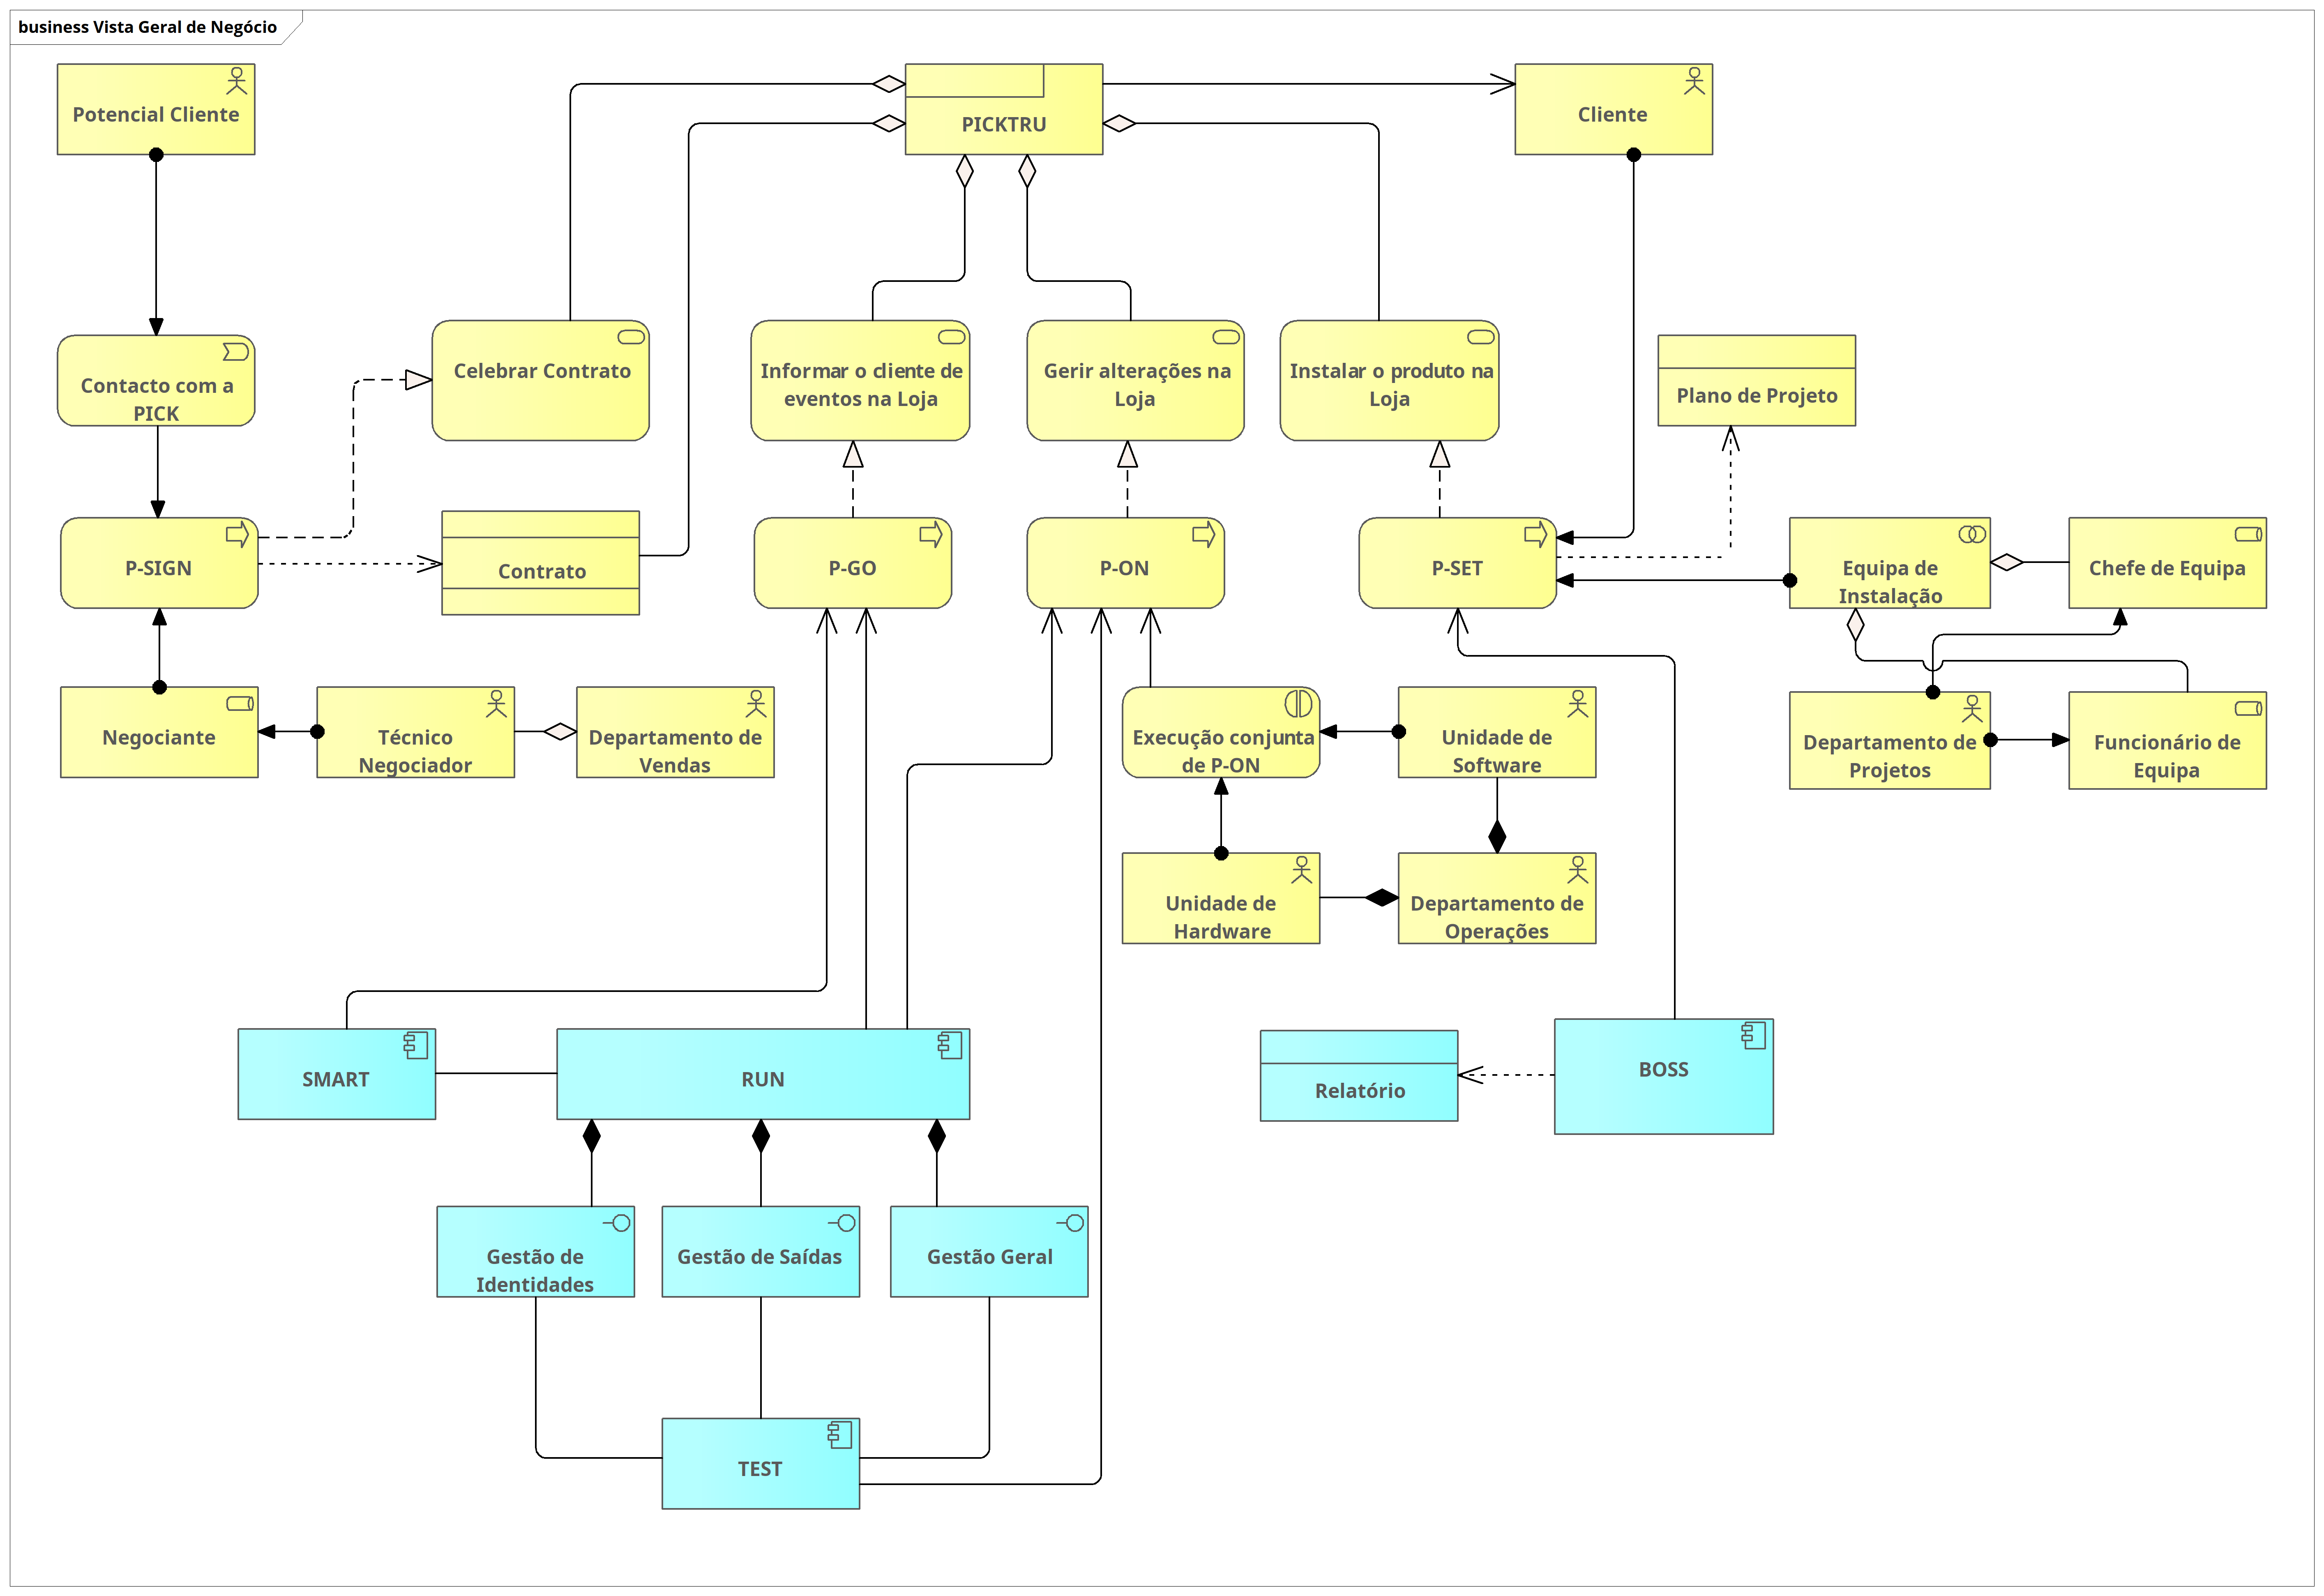
\includegraphics[width=1.4\textwidth]{assets/ea-archimate.png}
    \caption{(B.1.) Diagrama de Vista Geral do Negócio}
    \label{fig:archimate}
  \end{figure}
\end{landscape}

\begin{landscape}
  \begin{figure}
    \centering
    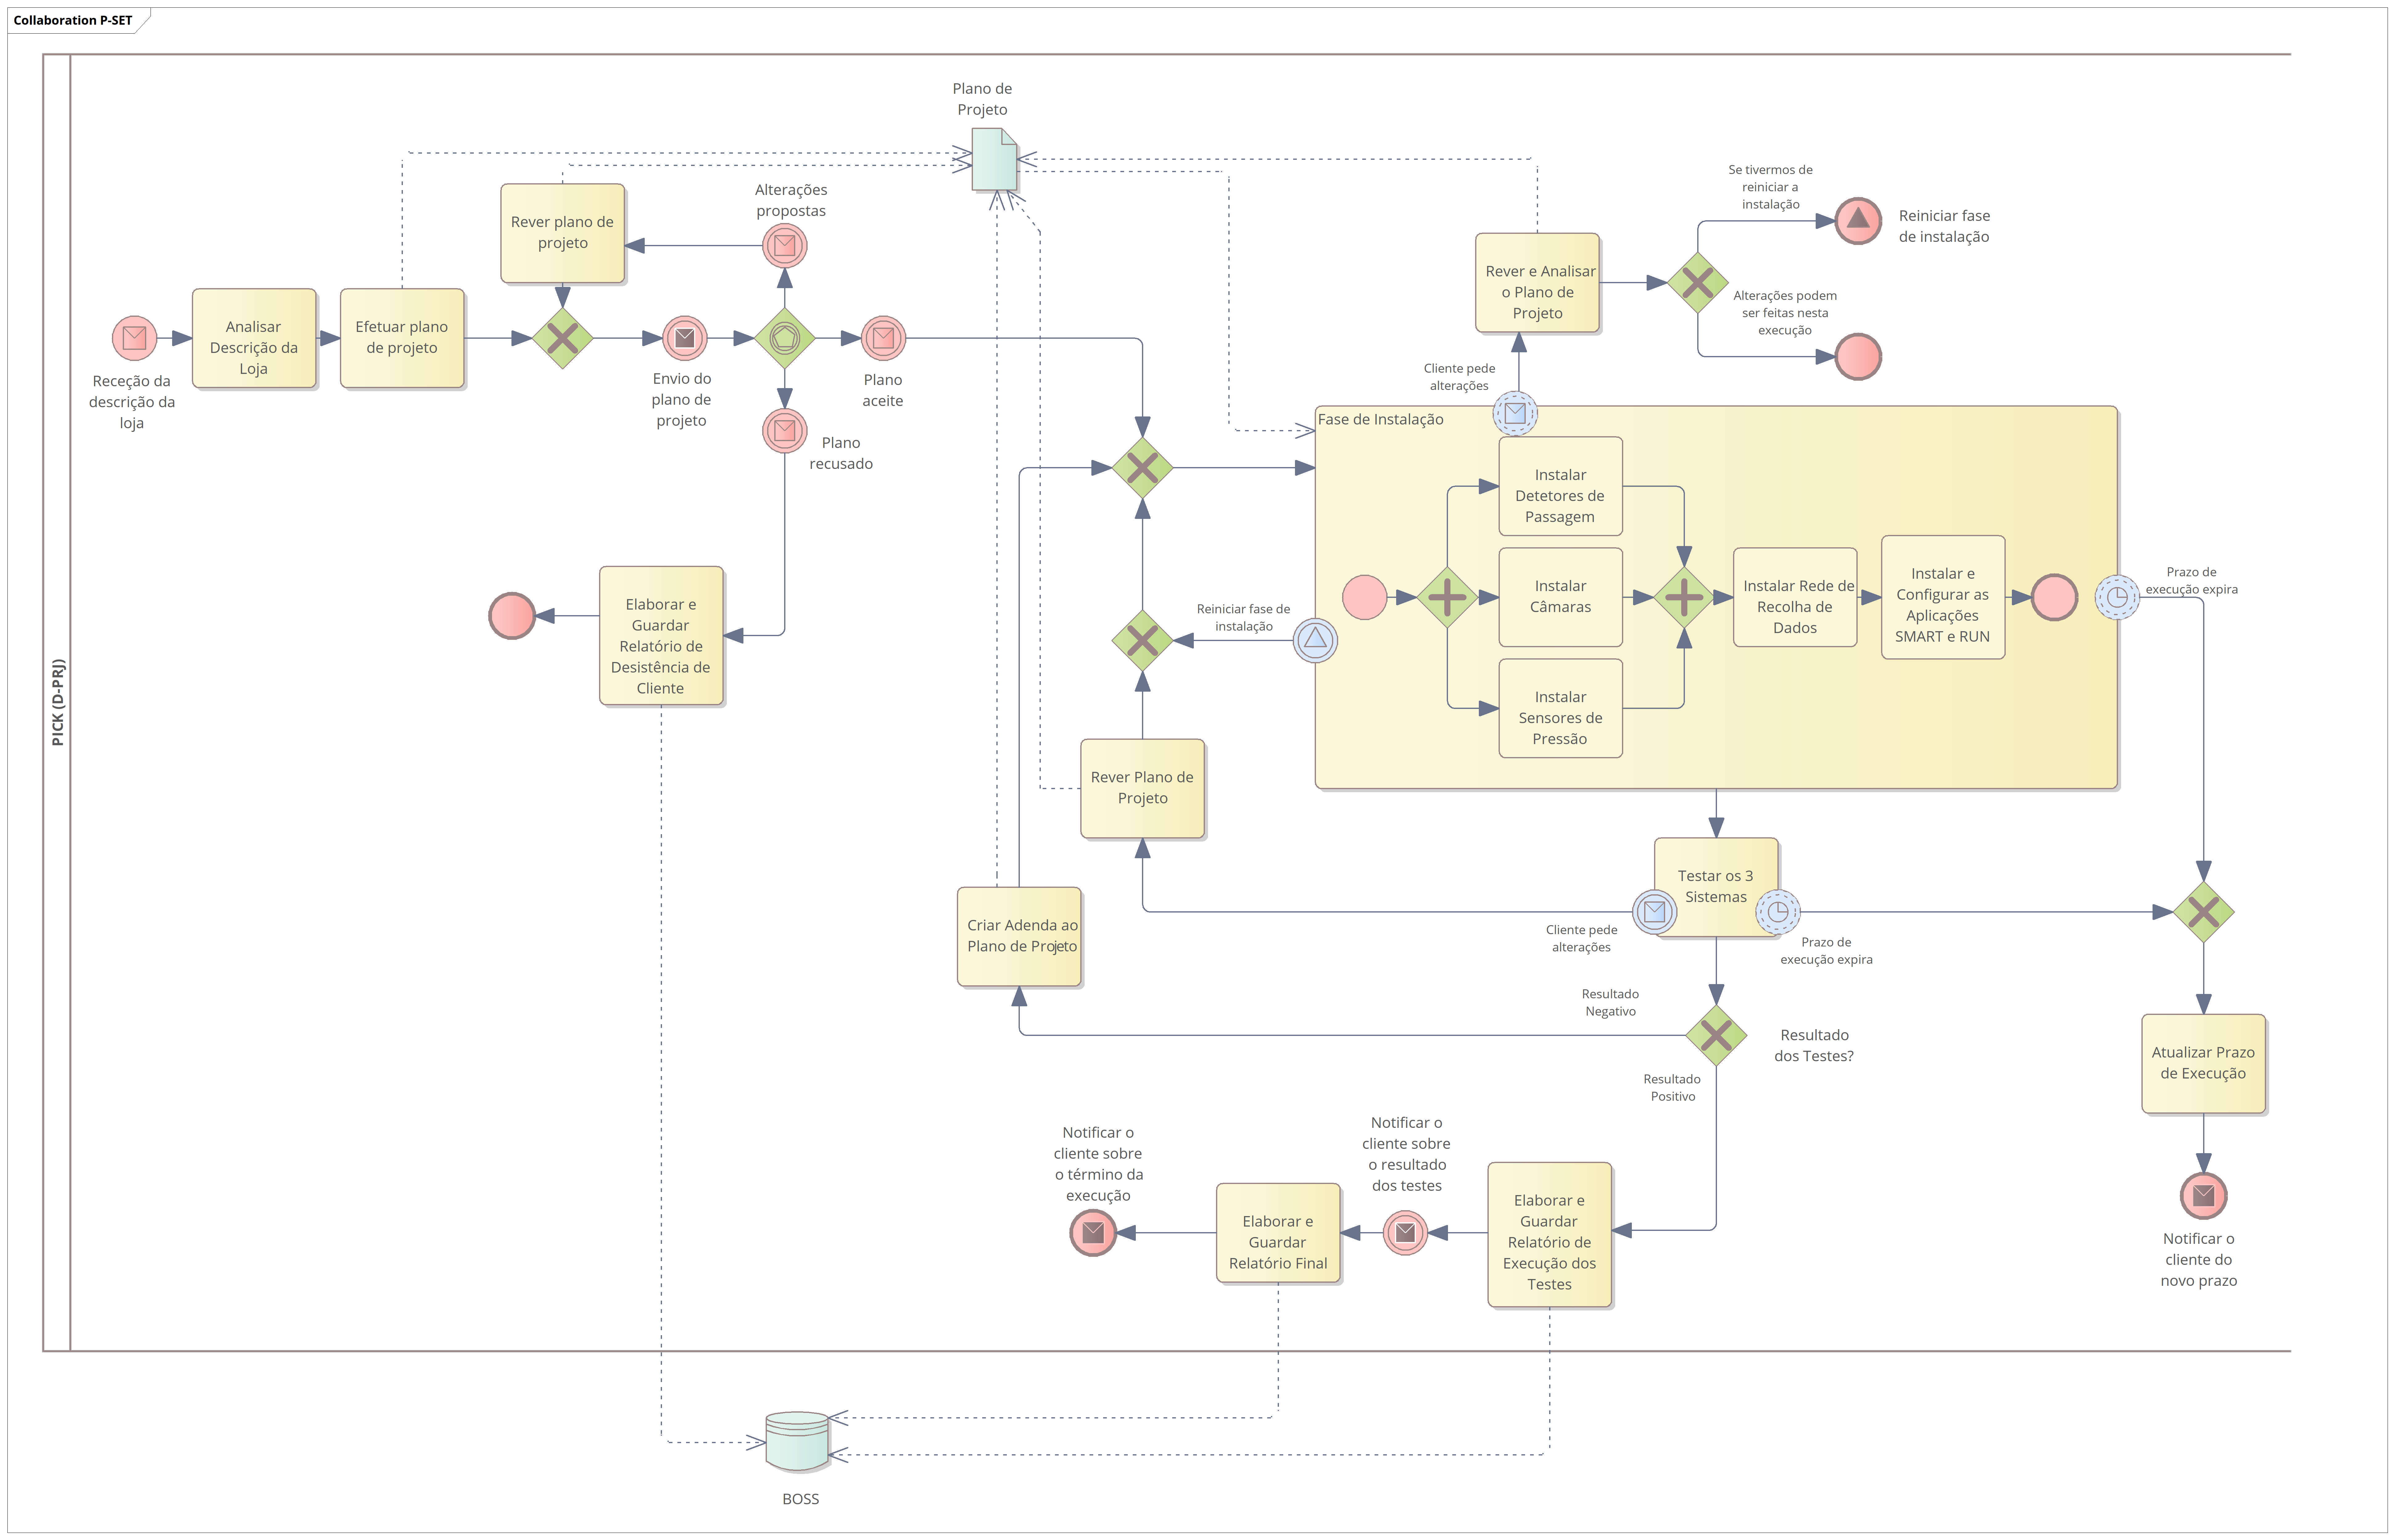
\includegraphics[width=1.5\textwidth]{assets/ea-p_set.png}
    \caption{(B.1.) Diagrama do Processo P-SET}
    \label{fig:p-set-bpmn}
  \end{figure}
\end{landscape}

\begin{landscape}
  \begin{figure}
    \centering
    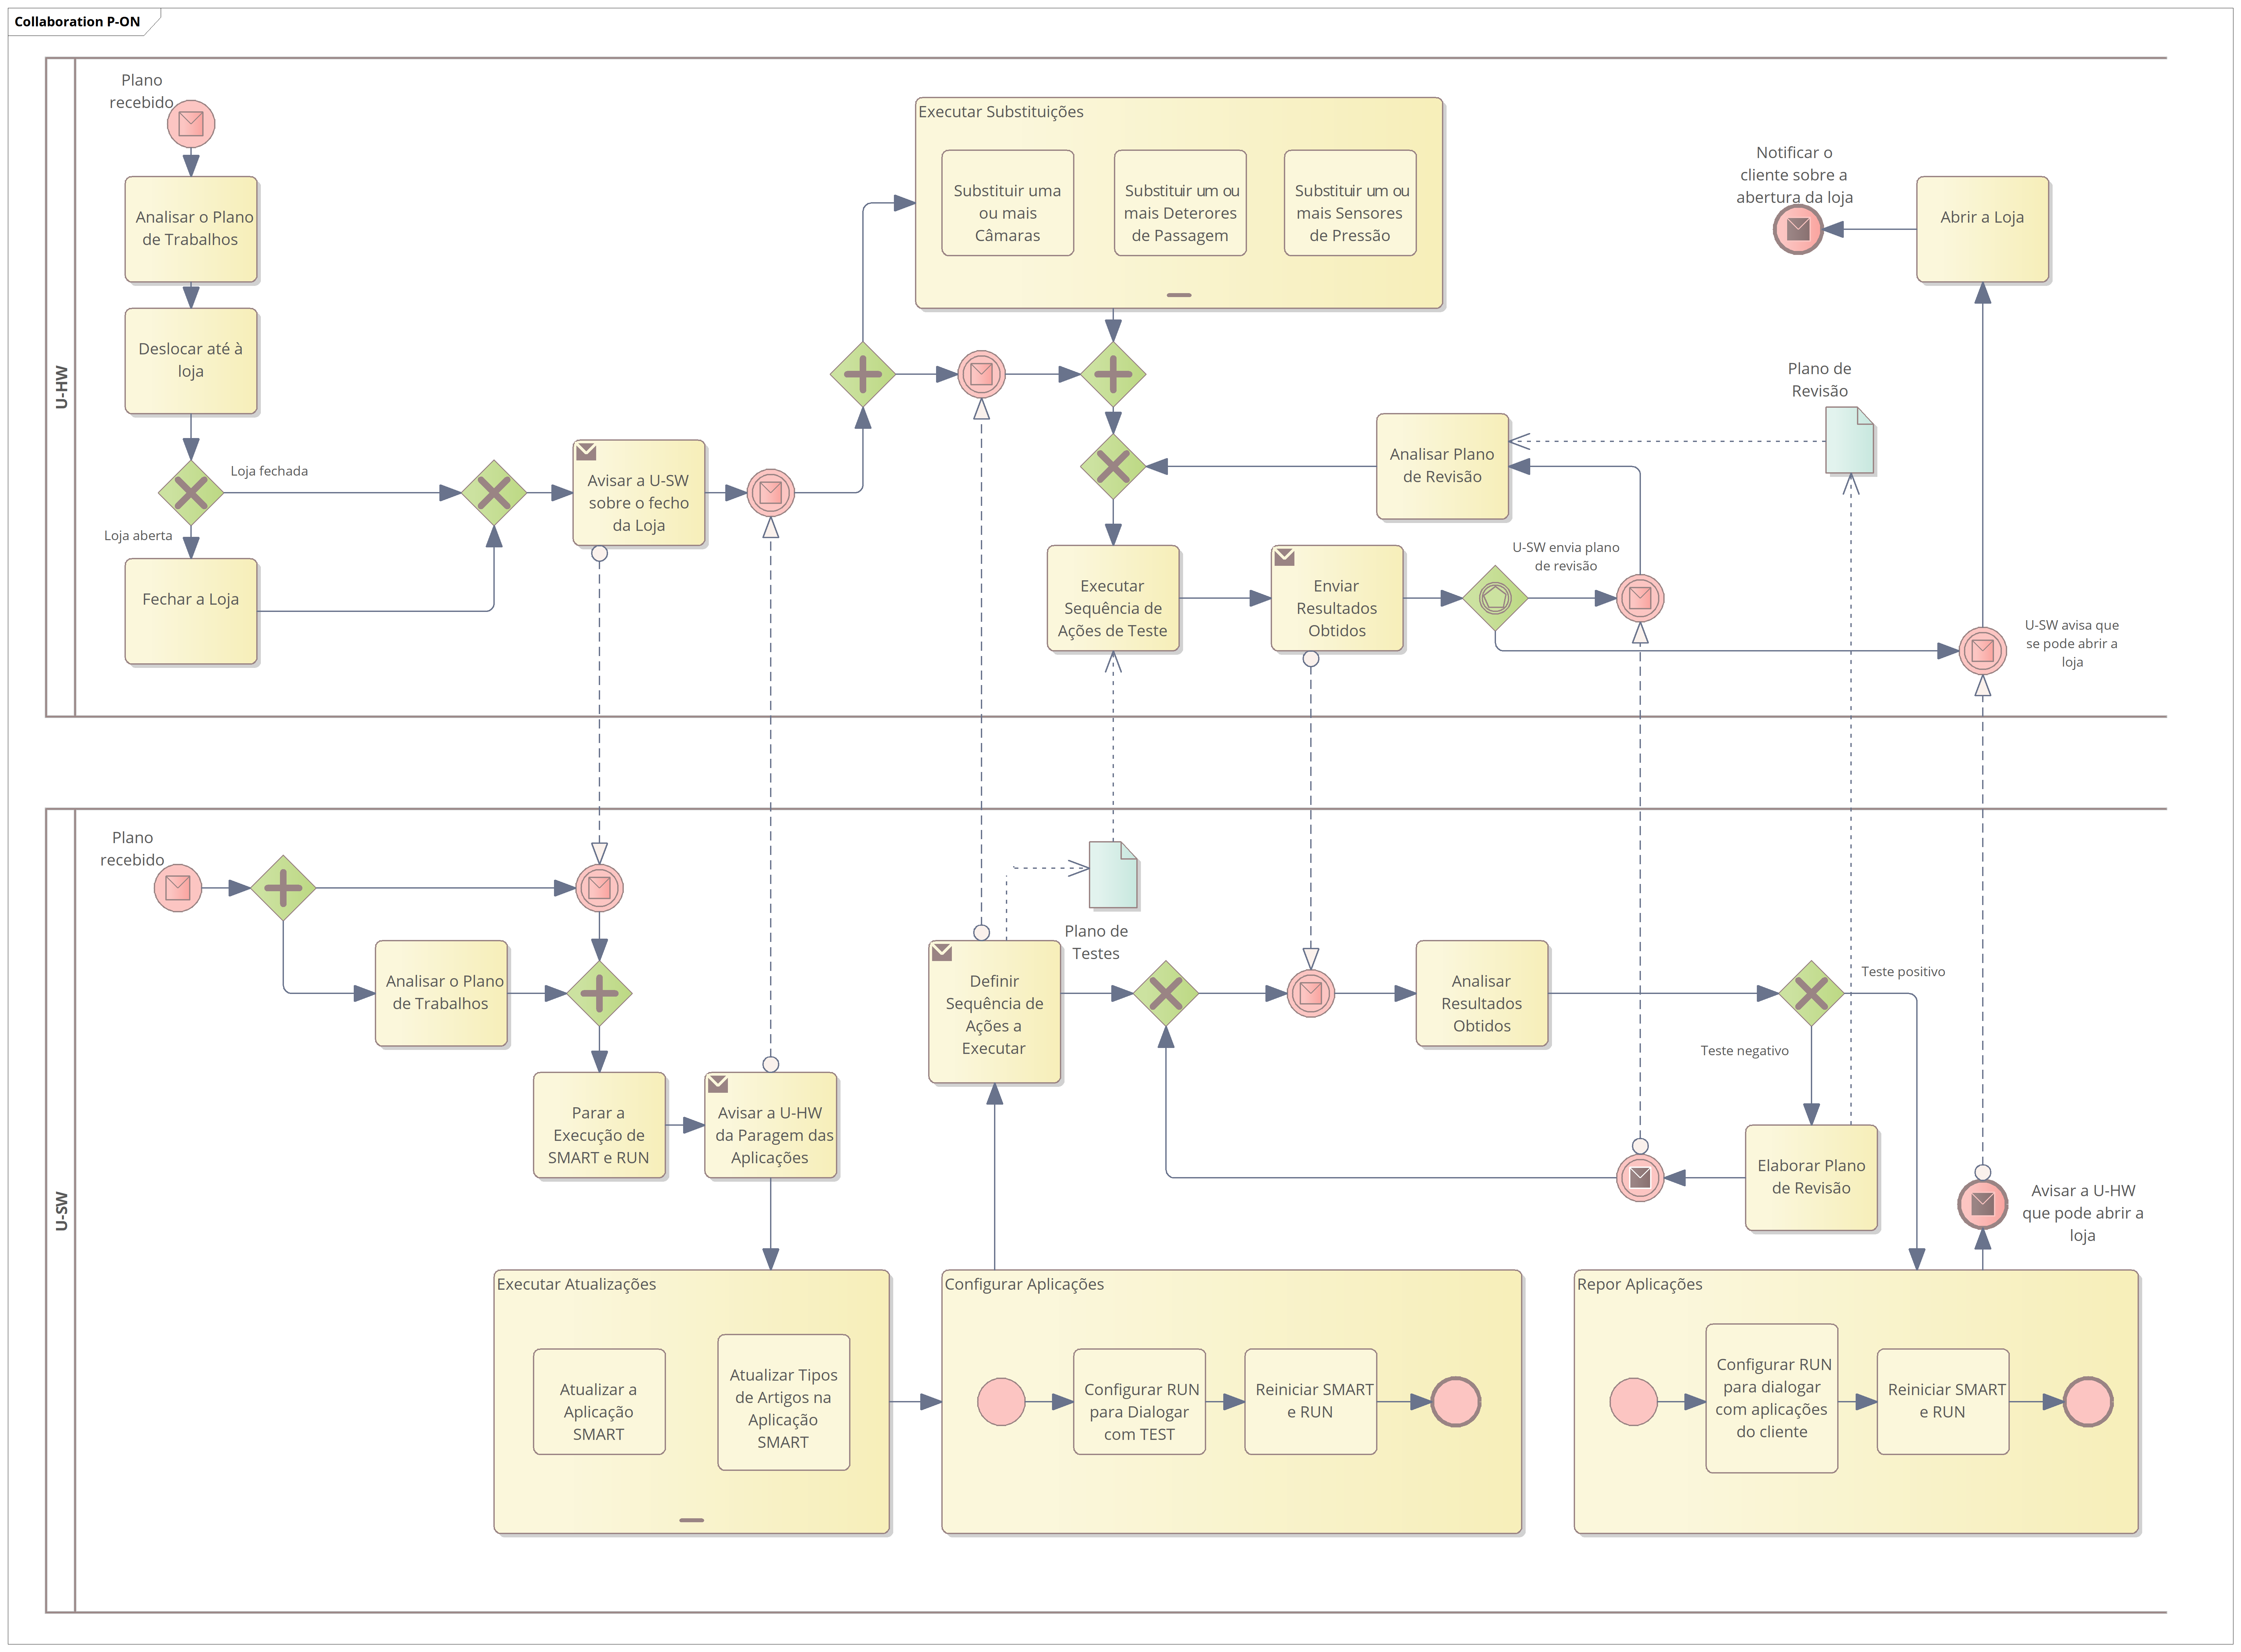
\includegraphics[width=1.35\textwidth]{assets/ea-p_on.png}
    \caption{(B.1.) Diagrama do Processo P-ON}
    \label{fig:p-on-bpmn}
  \end{figure}
\end{landscape}

\begin{landscape}
  \begin{figure}
    \centering
    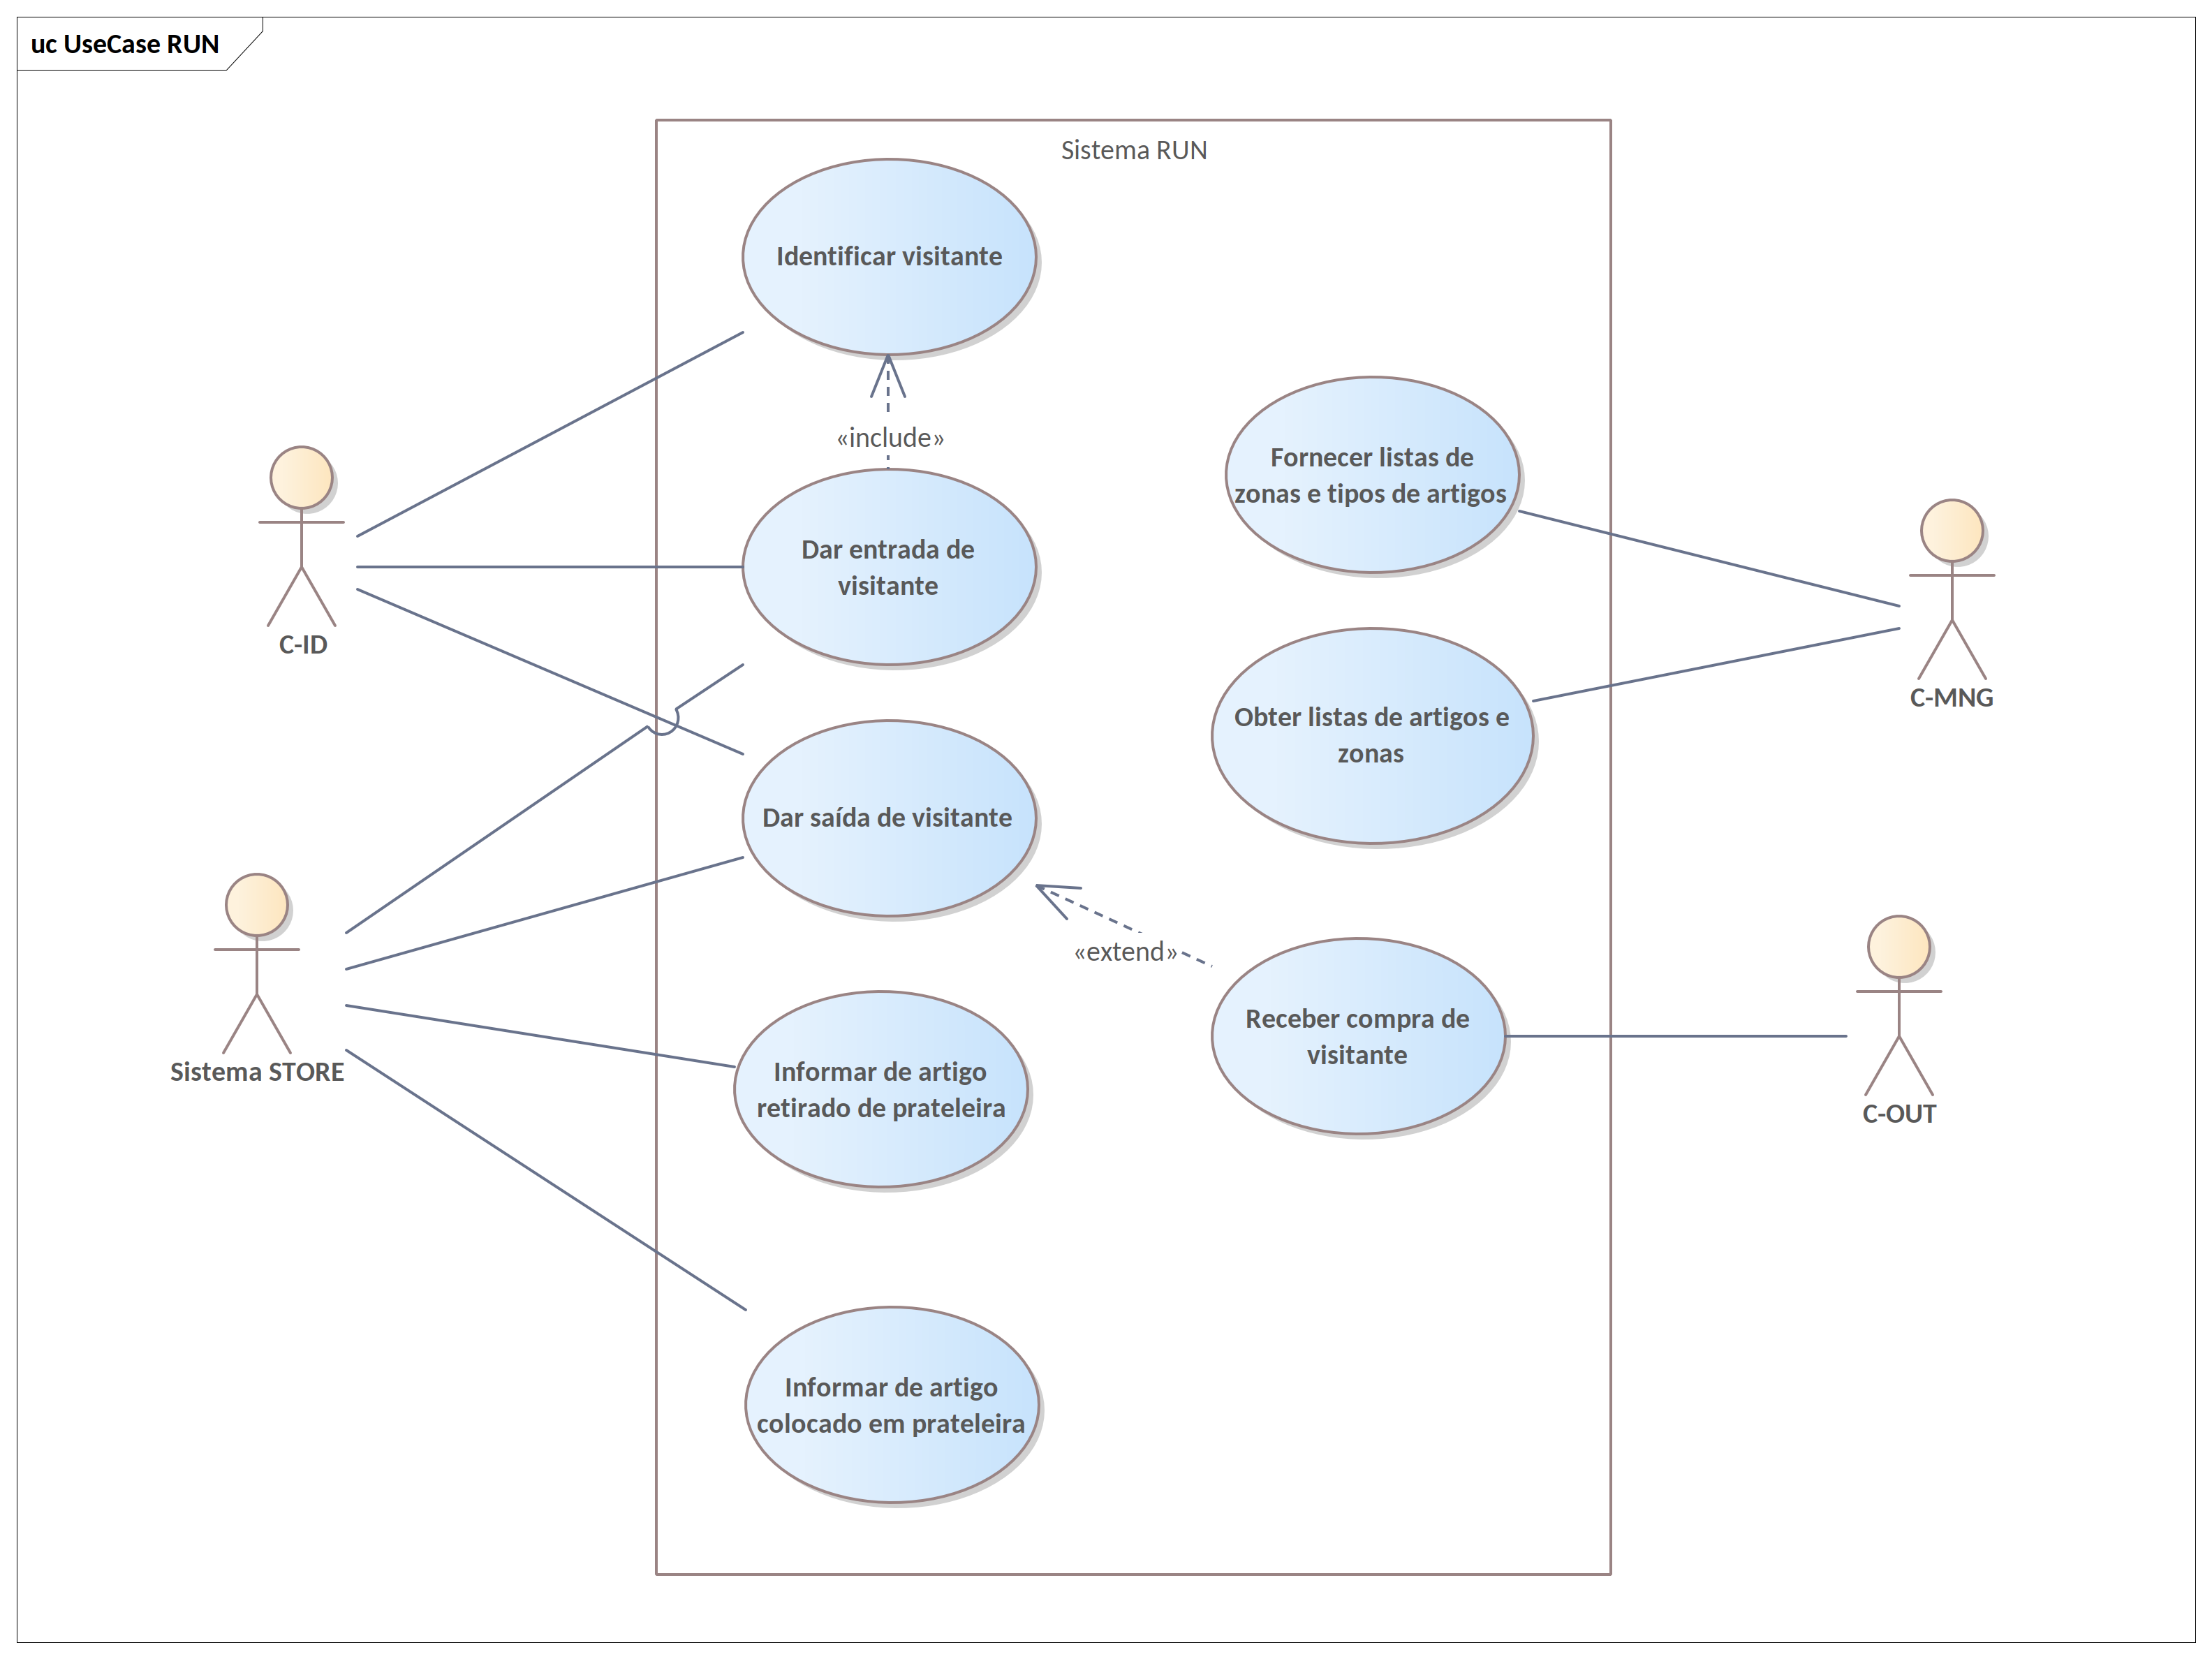
\includegraphics[width=1.3\textwidth]{assets/ea-usecase-run.png}
    \caption{(B.2.) Diagrama de Casos de Uso do sistema RUN}
    \label{fig:uc-run}
  \end{figure}
\end{landscape}

\begin{landscape}
  \begin{figure}
    \centering
    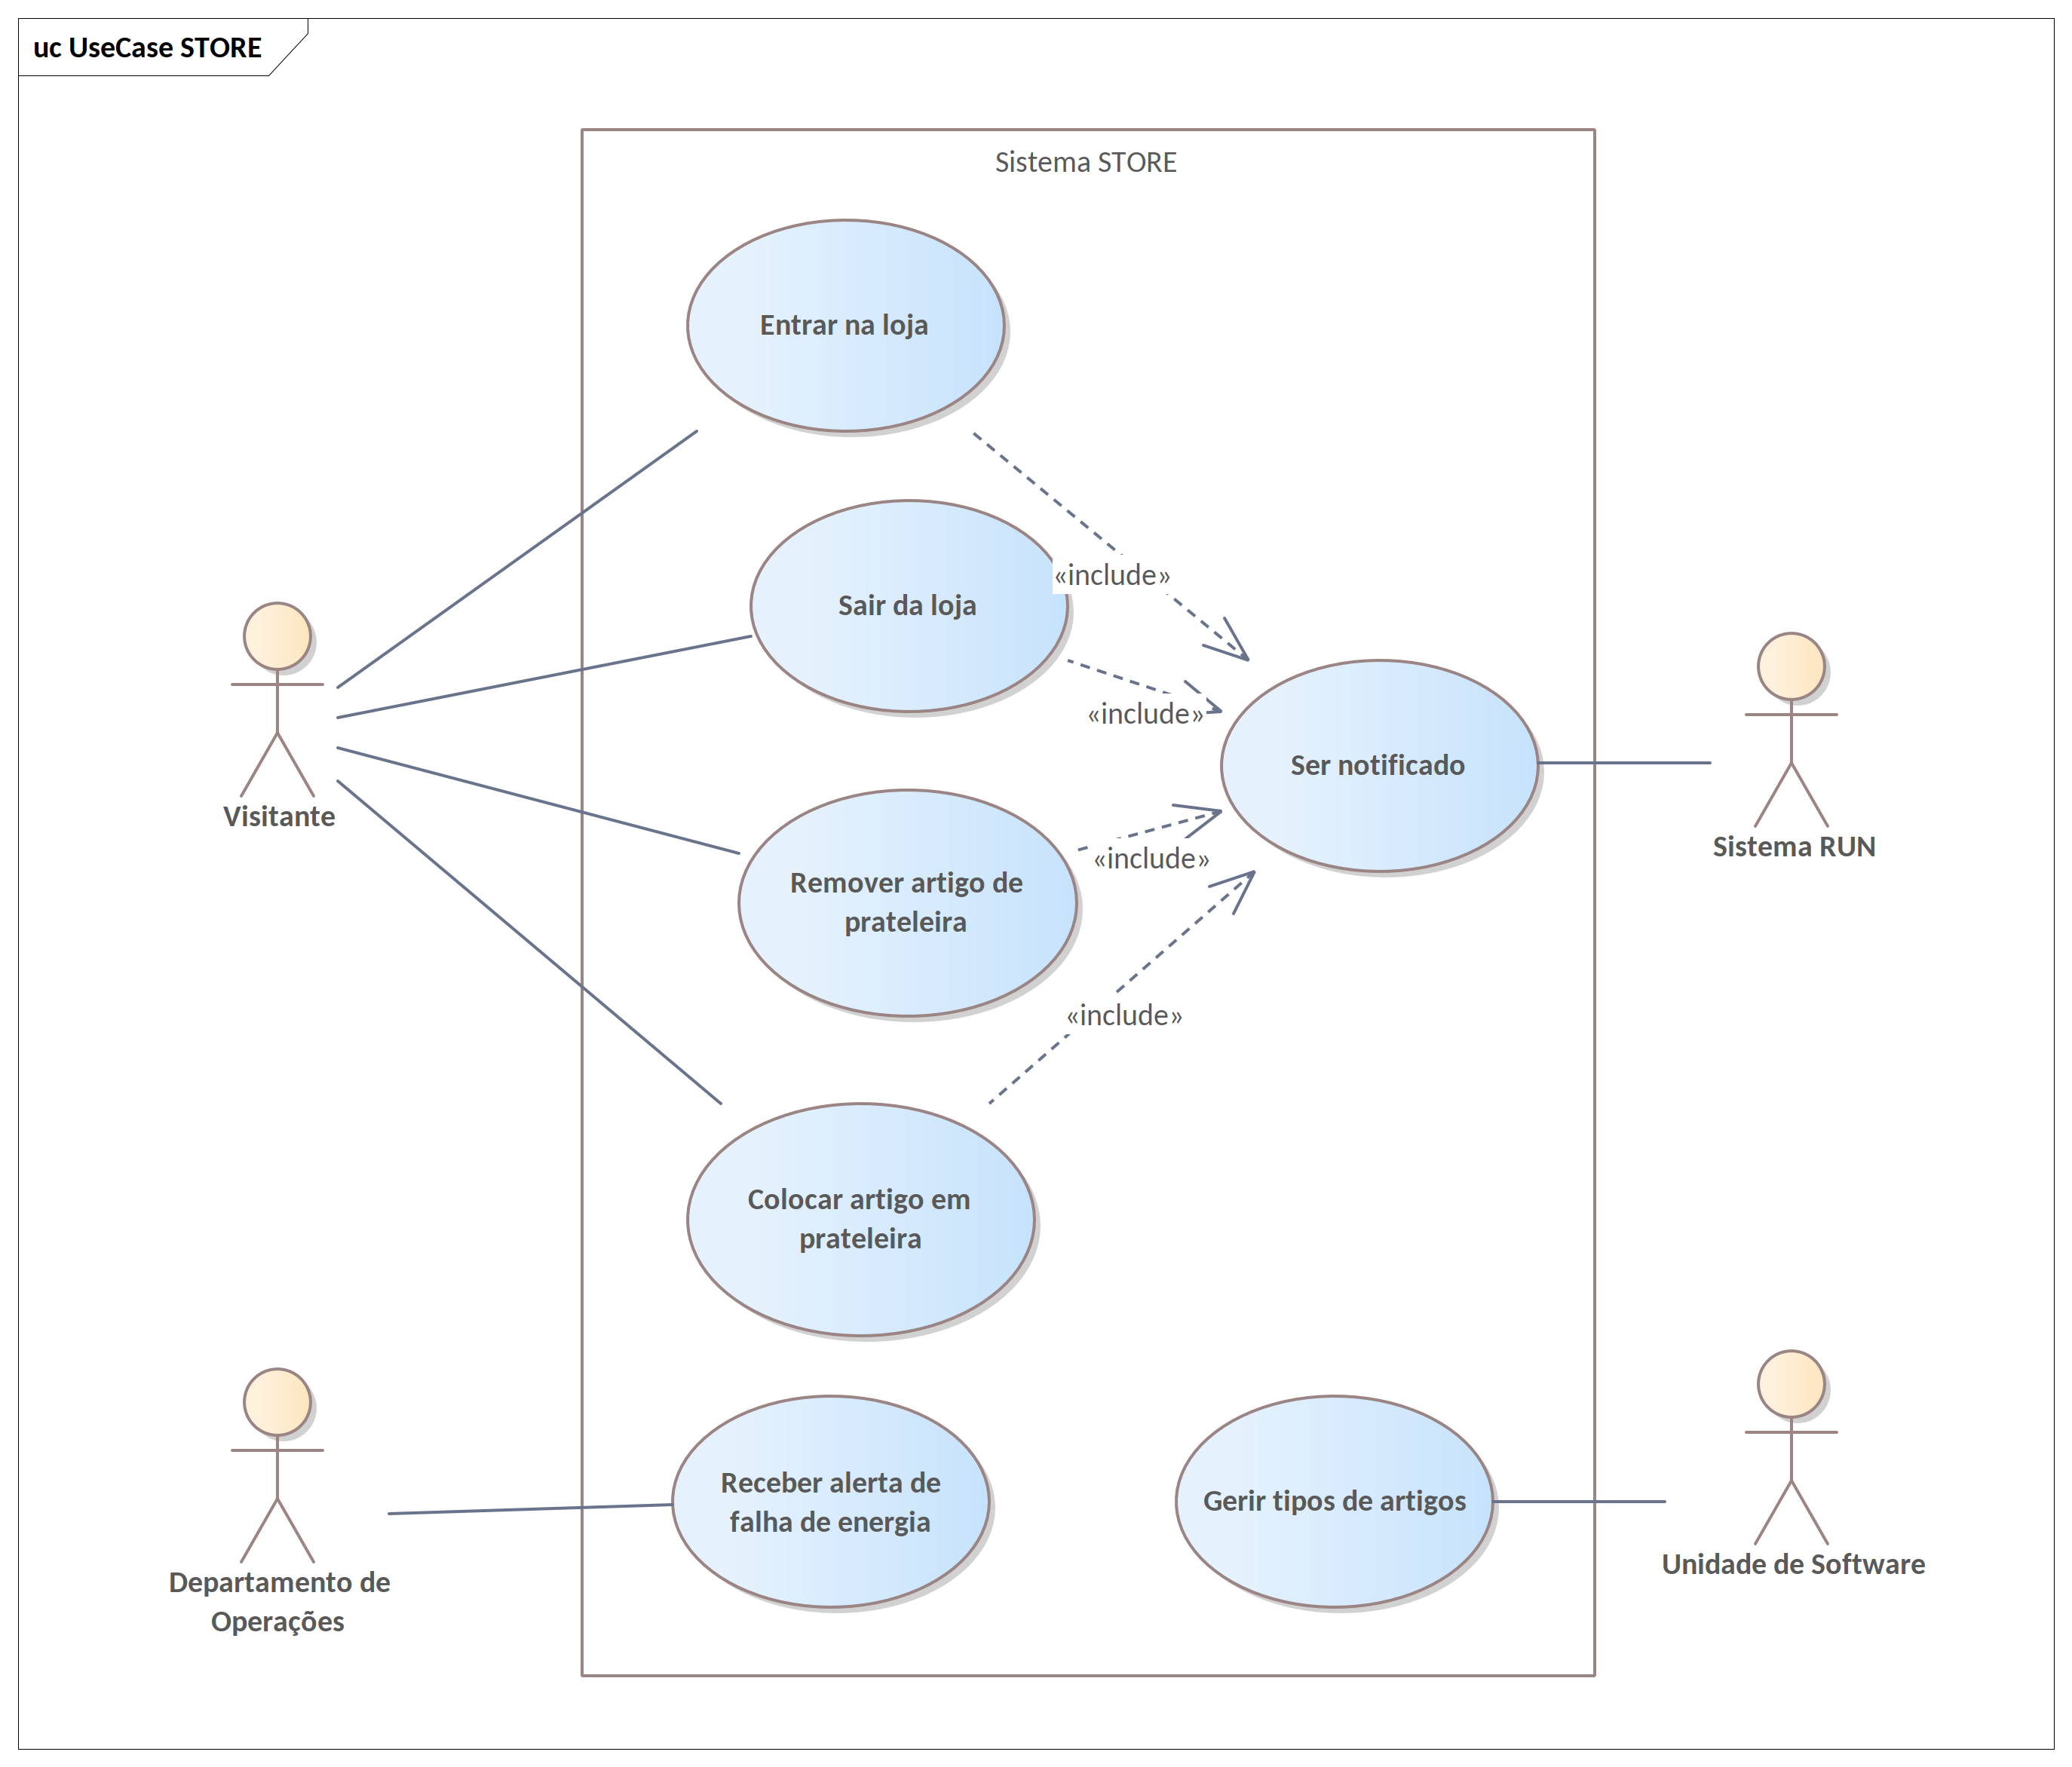
\includegraphics[width=1.15\textwidth]{assets/ea-usecase-store.png}
    \caption{(B.2.) Diagrama de Casos de Uso do sistema STORE}
    \label{fig:uc-store}
  \end{figure}
\end{landscape}

\begin{landscape}
  \begin{figure}
    \centering
    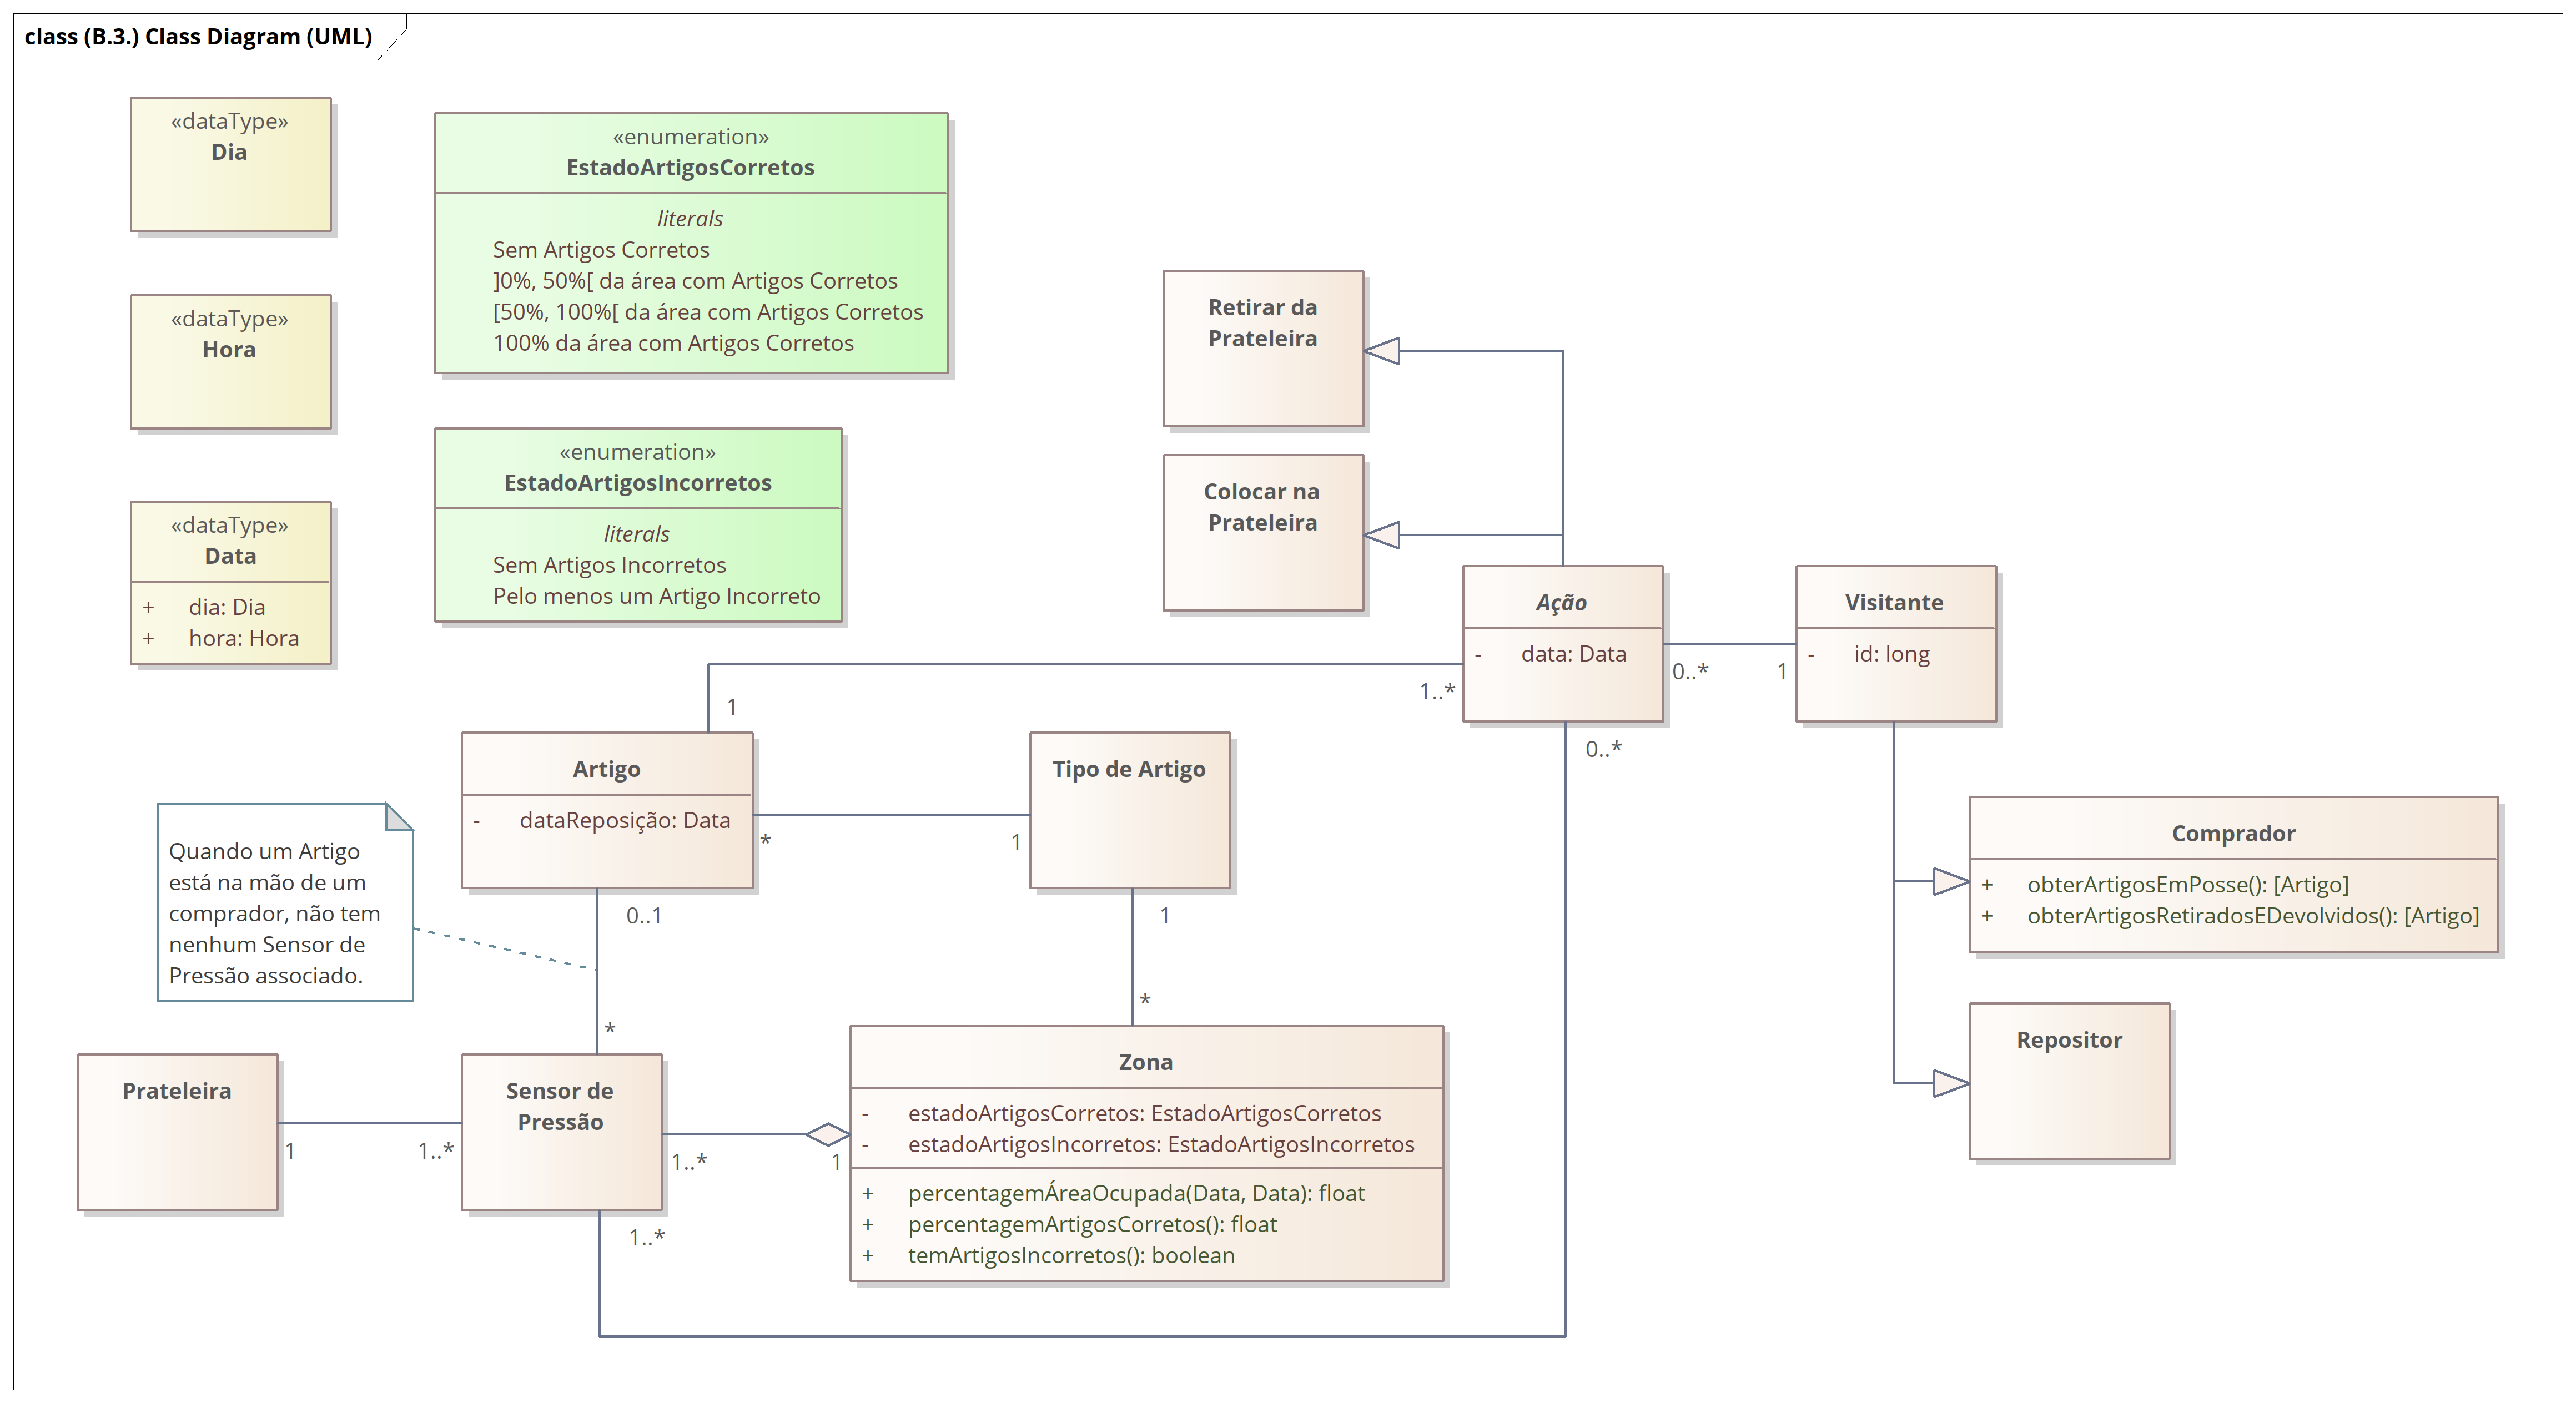
\includegraphics[width=1.6\textwidth]{assets/ea-uml.png}
    \caption{(B.3.) Diagrama de Classes (em UML) do modelo de domínio}
    \label{fig:uml}
  \end{figure}
\end{landscape}

\begin{landscape}
  \begin{figure}
    \centering
    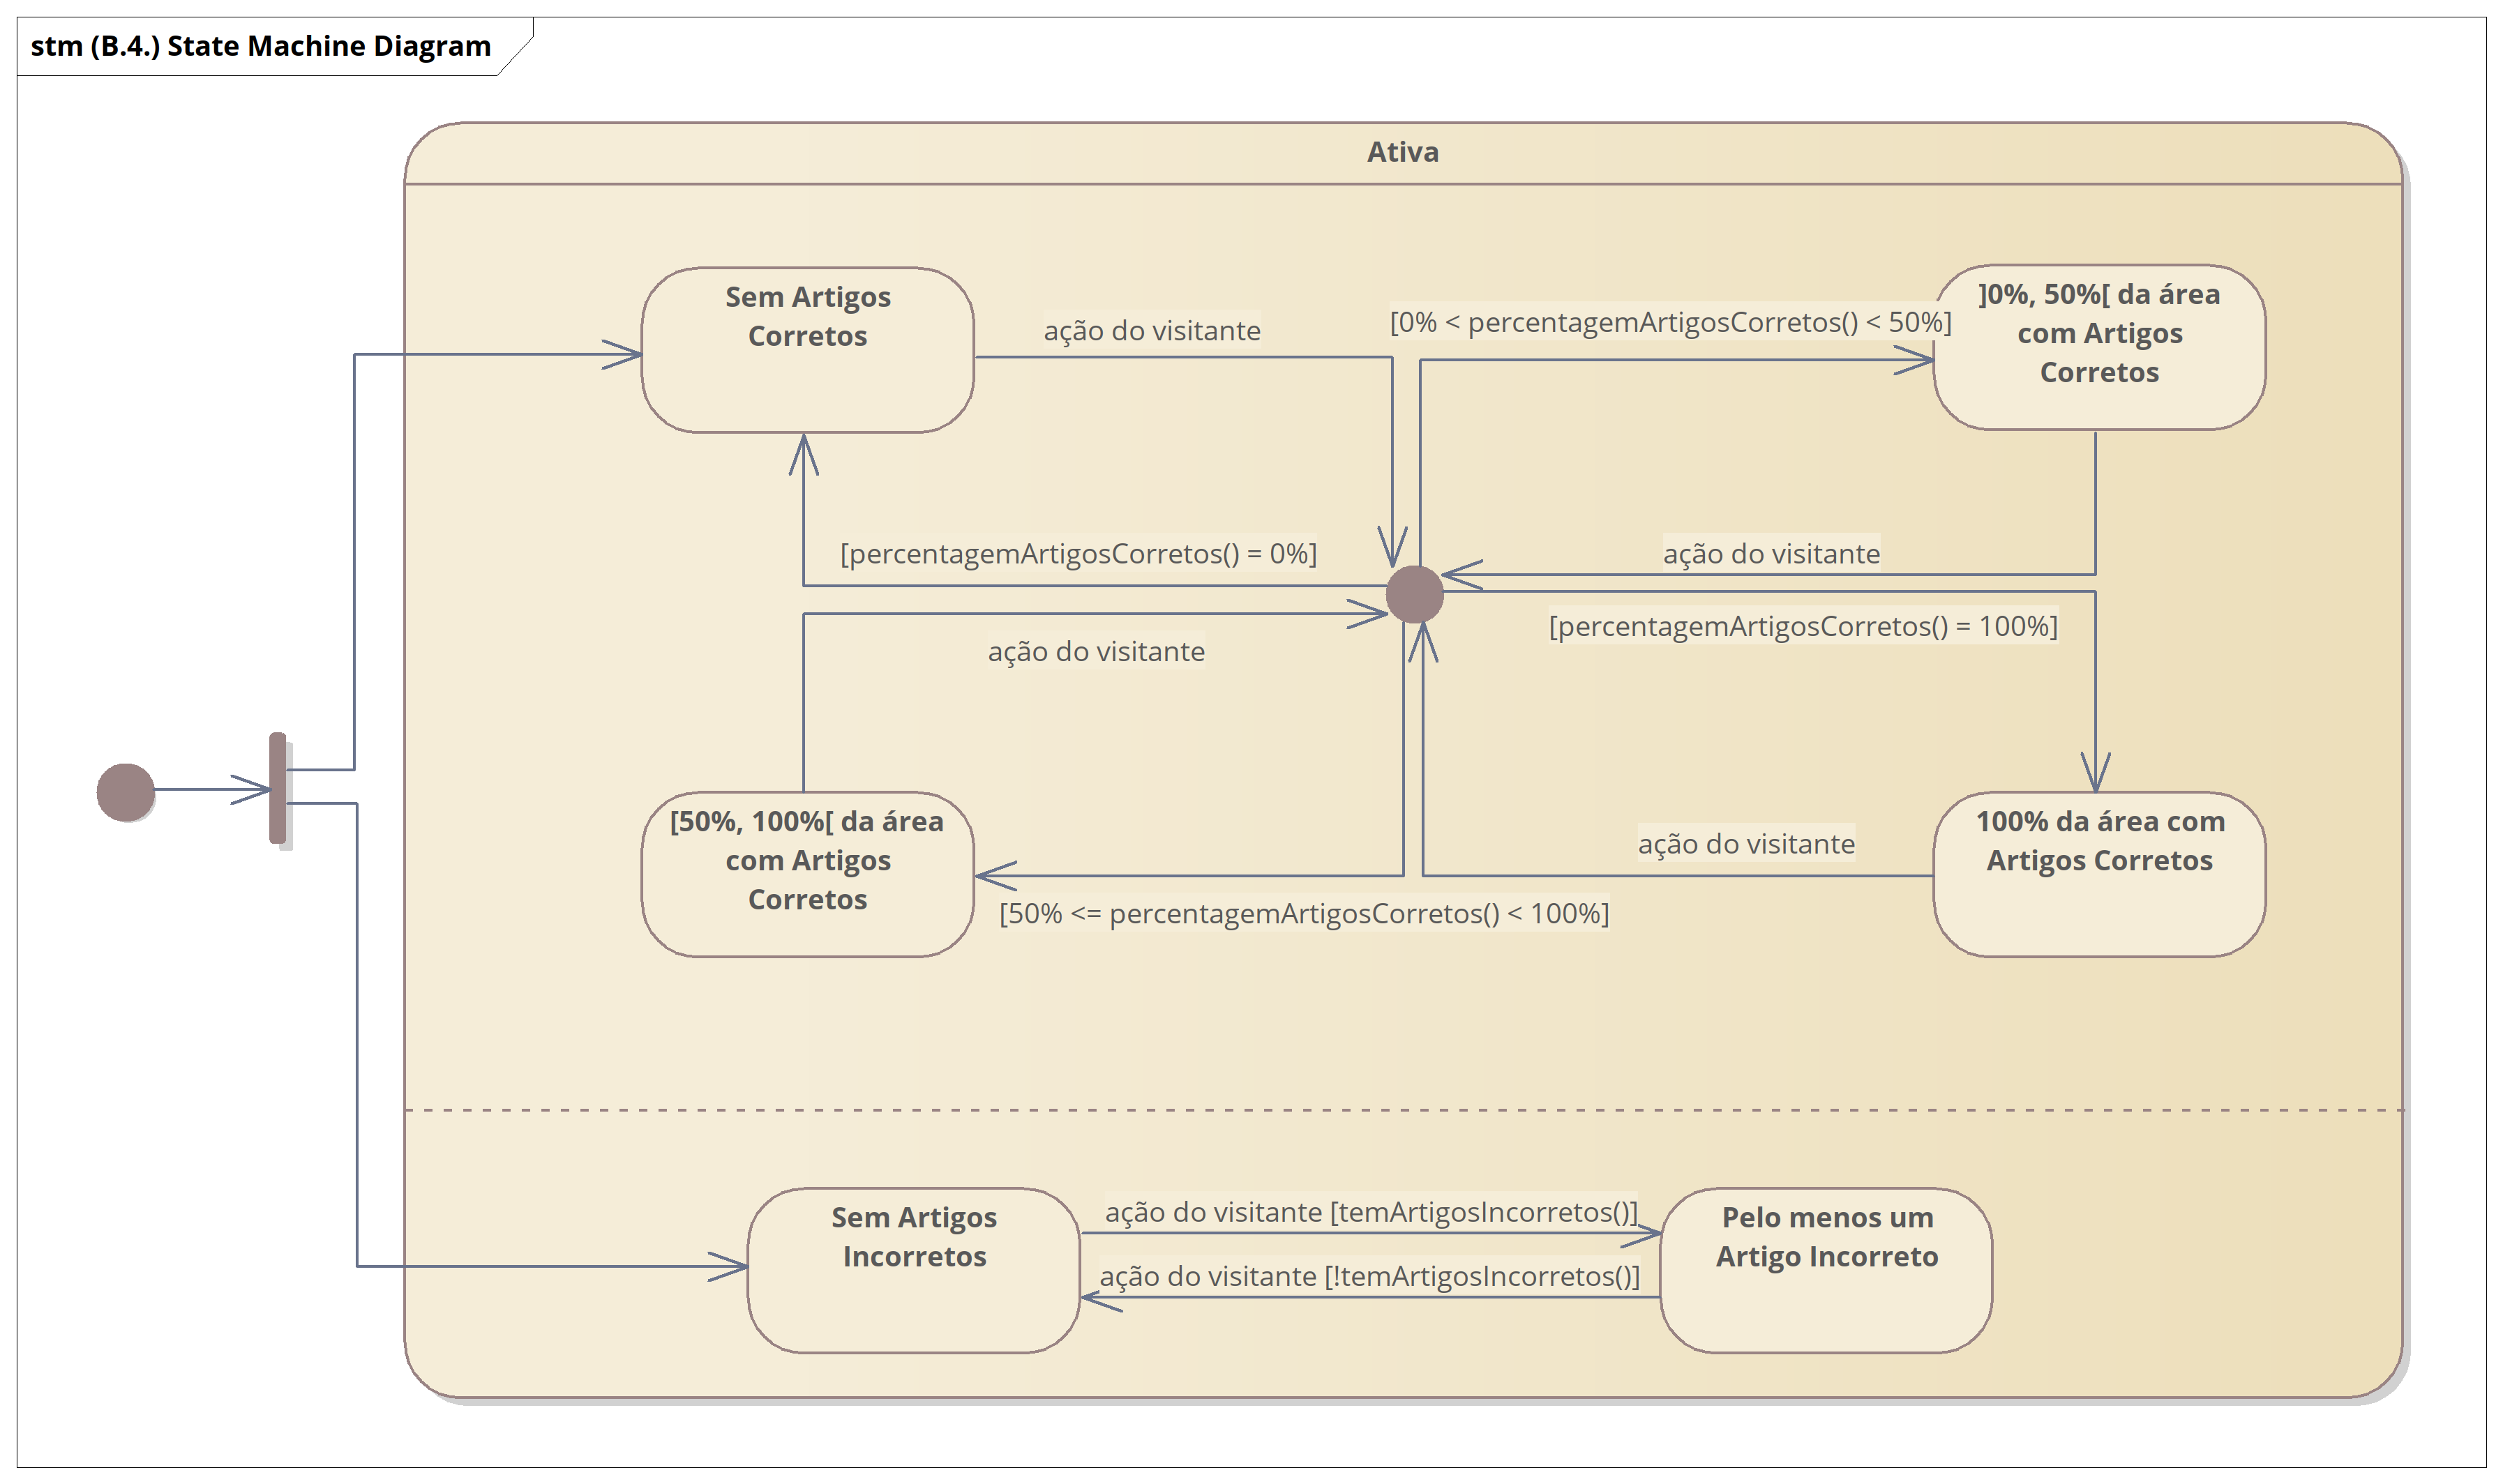
\includegraphics[width=1.6\textwidth]{assets/ea-state-machine.png}
    \caption{(B.4.) Diagrama de Máquina de Estados}
    \label{fig:state-machine}
  \end{figure}
\end{landscape}

\begin{landscape}
  \begin{figure}
    \centering
    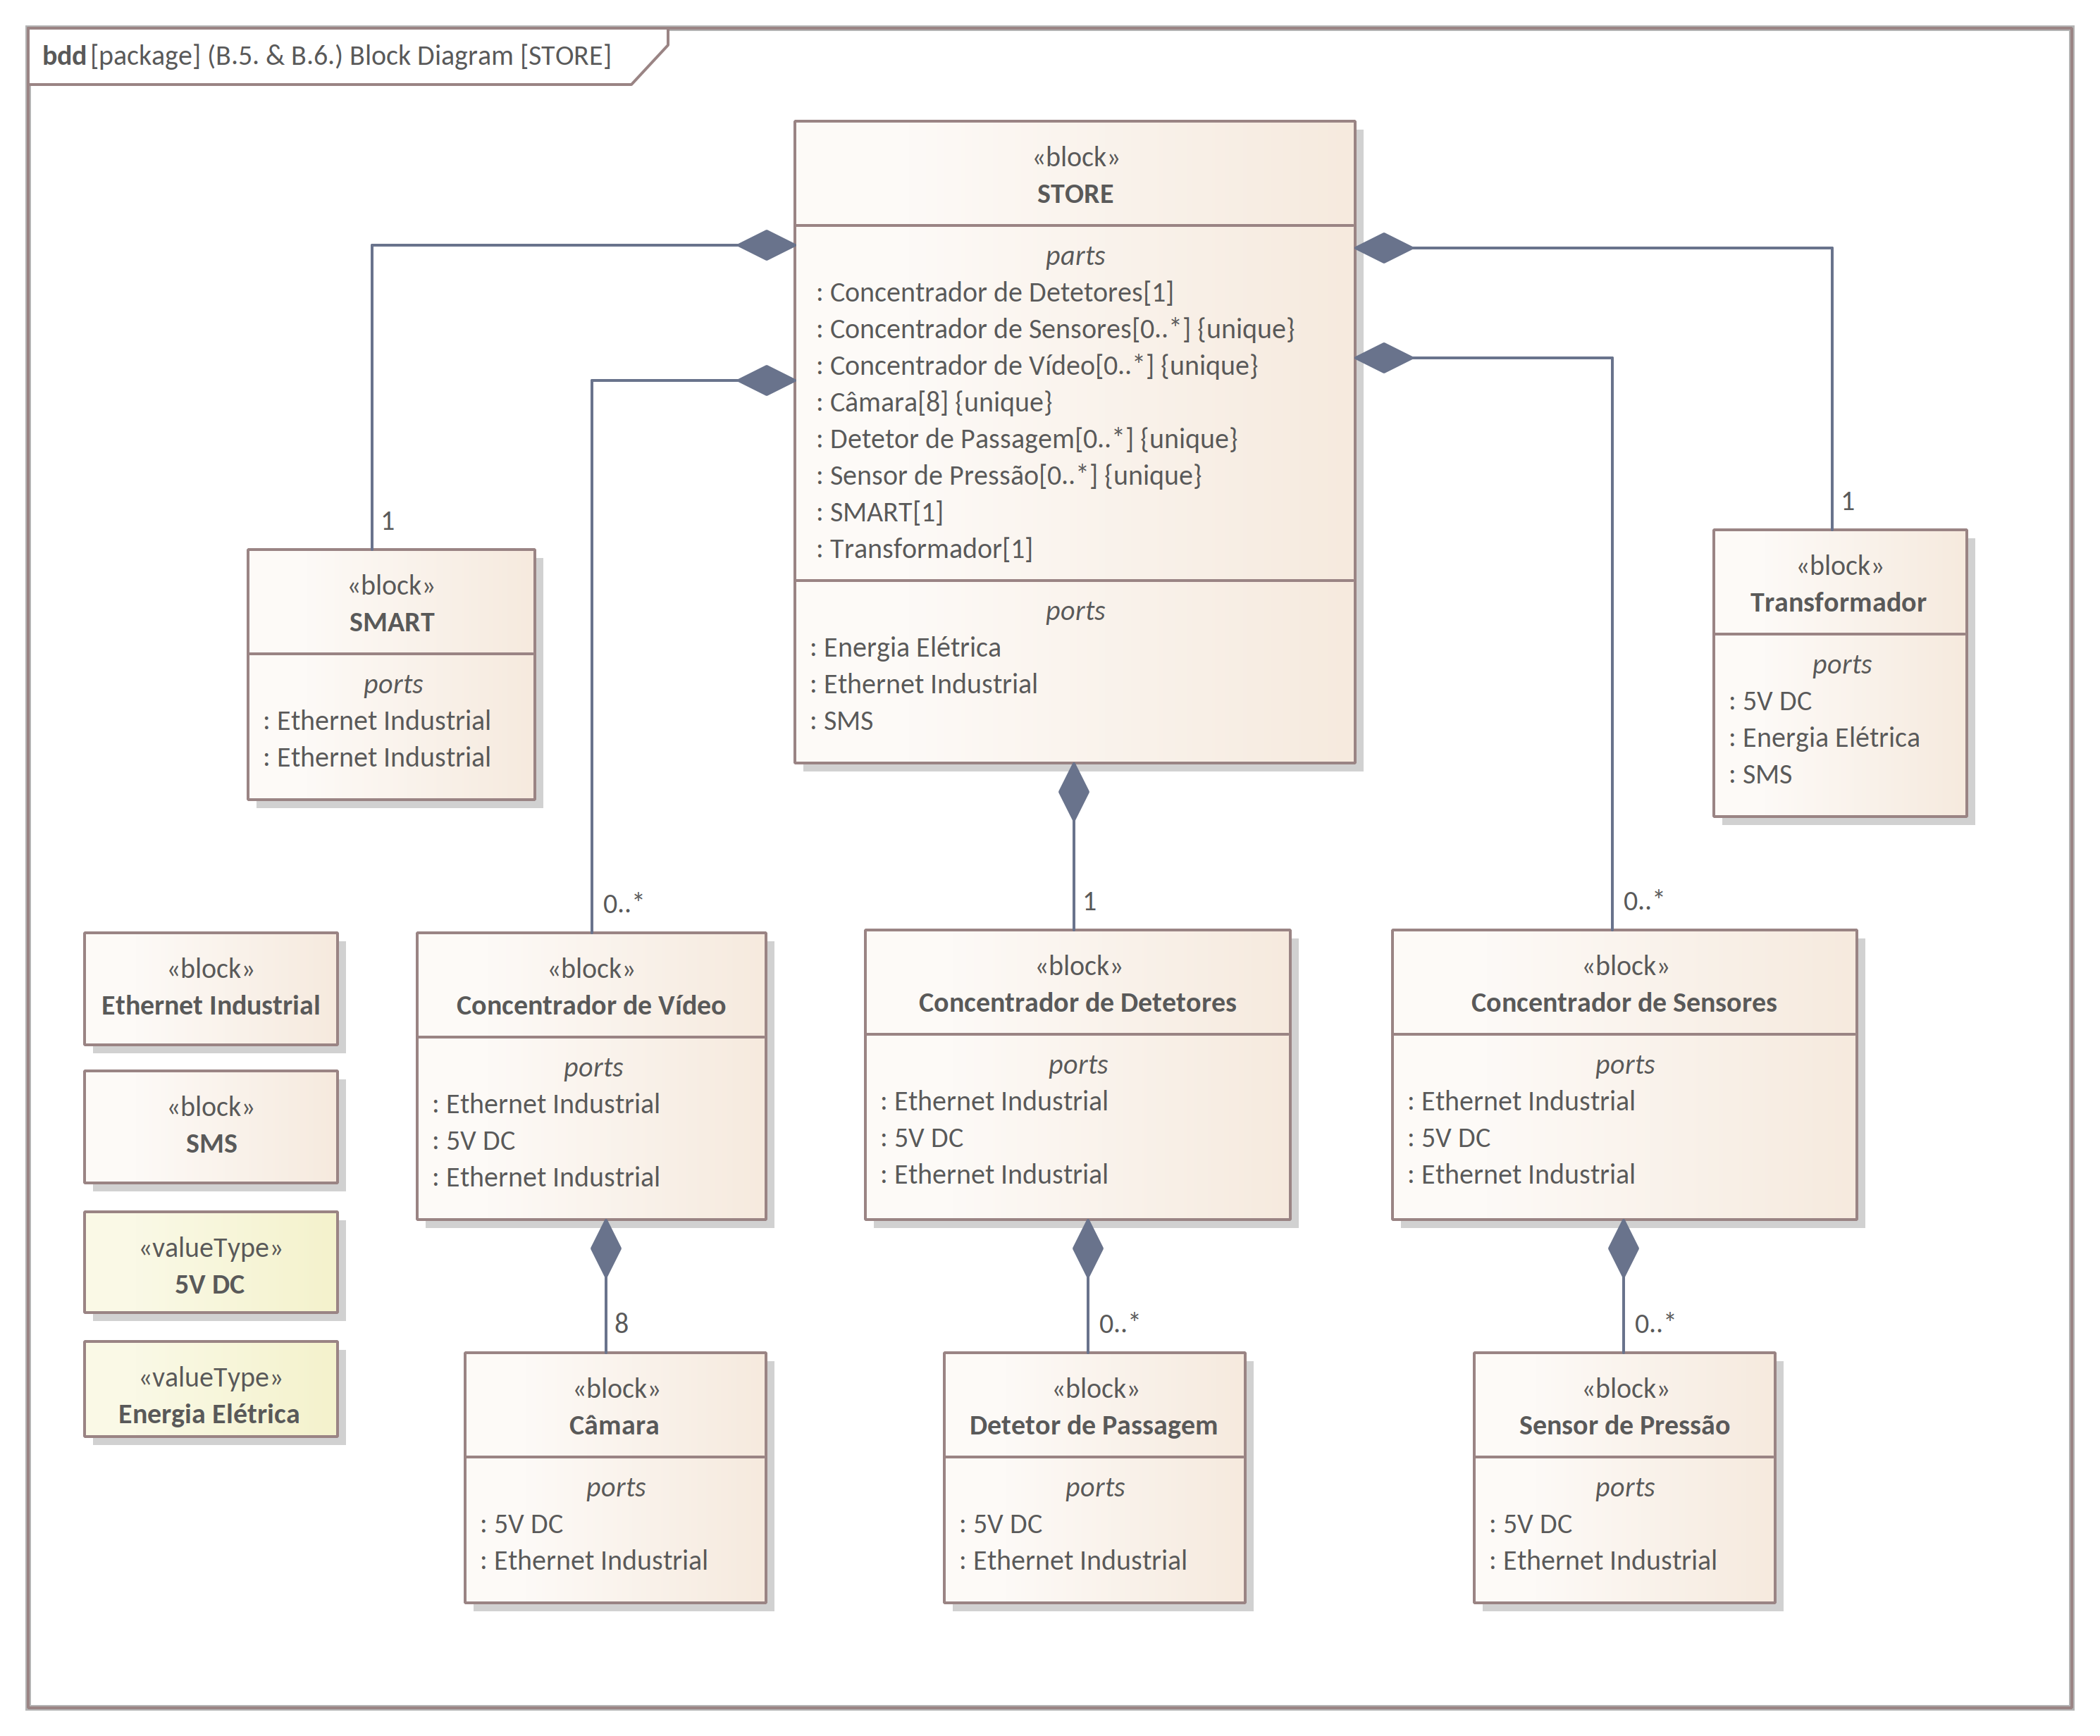
\includegraphics[width=1.2\textwidth]{assets/ea-bdd-store.png}
    \caption{(B.5.) Diagrama de Blocos}
    \label{fig:bbd}
  \end{figure}
\end{landscape}

\begin{landscape}
  \begin{figure}
    \centering
    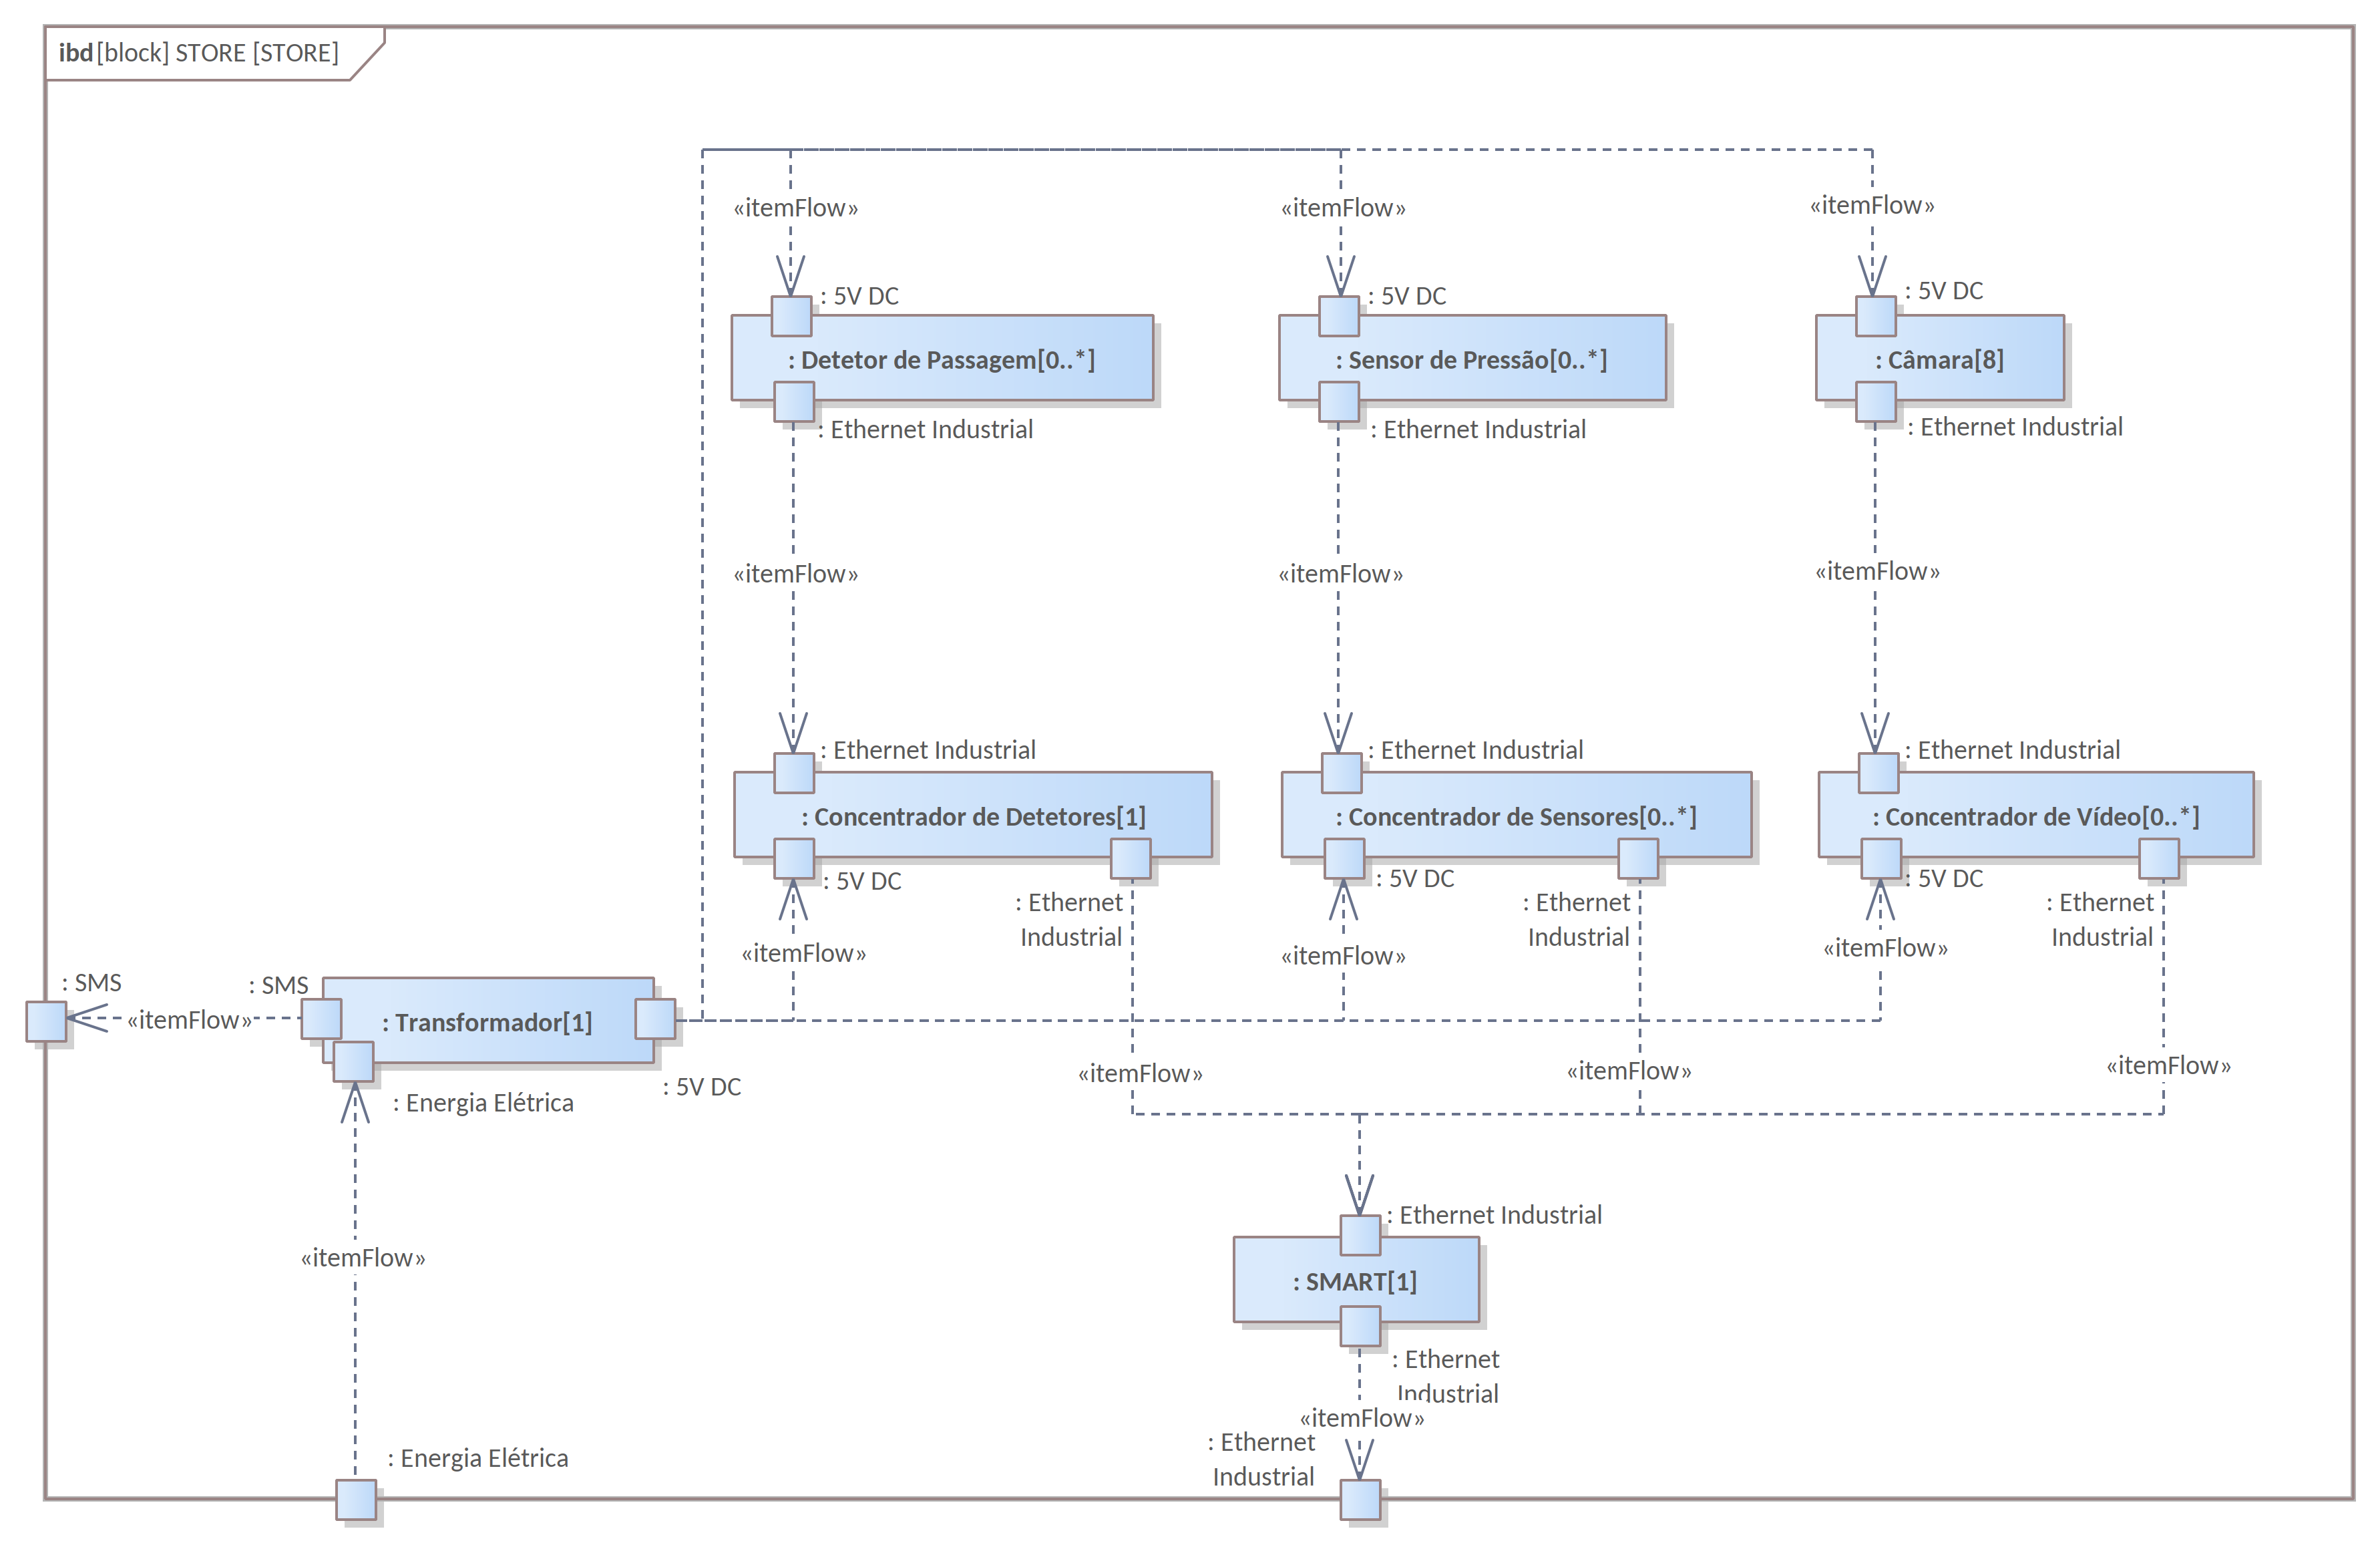
\includegraphics[width=1.5\textwidth]{assets/ea-ibd-store.png}
    \caption{(B.6. Diagrama Interno de Blocos)}
    \label{fig:ibd}
  \end{figure}
\end{landscape}

\end{document}